%% Copernicus Publications Manuscript Preparation Template for LaTeX Submissions
%% ---------------------------------
%% This template should be used for copernicus.cls
%% The class file and some style files are bundled in the Copernicus Latex Package, which can be downloaded from the different journal webpages.
%% For further assistance please contact Copernicus Publications at: production@copernicus.org
%% https://publications.copernicus.org/for_authors/manuscript_preparation.html


%% Please use the following documentclass and journal abbreviations for discussion papers and final revised papers.

%% 2-column papers and discussion papers
\documentclass[journal abbreviation, manuscript]{copernicus}



%% Journal abbreviations (please use the same for discussion papers and final revised papers)


% Advances in Geosciences (adgeo)
% Advances in Radio Science (ars)
% Advances in Science and Research (asr)
% Advances in Statistical Climatology, Meteorology and Oceanography (ascmo)
% Annales Geophysicae (angeo)
% Archives Animal Breeding (aab)
% ASTRA Proceedings (ap)
% Atmospheric Chemistry and Physics (acp)
% Atmospheric Measurement Techniques (amt)
% Biogeosciences (bg)
% Climate of the Past (cp)
% DEUQUA Special Publications (deuquasp)
% Drinking Water Engineering and Science (dwes)
% Earth Surface Dynamics (esurf)
% Earth System Dynamics (esd)
% Earth System Science Data (essd)
% E&G Quaternary Science Journal (egqsj)
% European Journal of Mineralogy (ejm)
% Fossil Record (fr)
% Geochronology (gchron)
% Geographica Helvetica (gh)
% Geoscience Communication (gc)
% Geoscientific Instrumentation, Methods and Data Systems (gi)
% Geoscientific Model Development (gmd)
% History of Geo- and Space Sciences (hgss)
% Hydrology and Earth System Sciences (hess)
% Journal of Micropalaeontology (jm)
% Journal of Sensors and Sensor Systems (jsss)
% Mechanical Sciences (ms)
% Natural Hazards and Earth System Sciences (nhess)
% Nonlinear Processes in Geophysics (npg)
% Ocean Science (os)
% Primate Biology (pb)
% Proceedings of the International Association of Hydrological Sciences (piahs)
% Scientific Drilling (sd)
% SOIL (soil)
% Solid Earth (se)
% The Cryosphere (tc)
% Weather and Climate Dynamics (wcd)
% Web Ecology (we)
% Wind Energy Science (wes)


%% \usepackage commands included in the copernicus.cls:
%\usepackage[german, english]{babel}
\usepackage{tabularx}
%\usepackage{cancel}
\usepackage{multirow}
%\usepackage{supertabular}
%\usepackage{algorithmic}
%\usepackage{algorithm}
%\usepackage{amsthm}
%\usepackage{float}
%\usepackage{subfig}
%\usepackage{rotating}

\usepackage{booktabs}
%\usepackage{longtable}
%\usepackage{ltablex}

\begin{document}

\title{Do the  climate models reproduce the observed aerosol trends over the last two decades?}

% \Author[affil]{given_name}{surname}
\Author[1]{Augustin}{Mortier}
\Author[1]{Jonas}{Gliss}
\Author[1]{Michael}{Schulz}

\Author[2]{others}{}
\affil[1]{Norwegian Meteorological Institute}
\affil[2]{ADDRESS}

%co-authors/references:
%ECMWF Rean:
%NorESM2: Alf and Dirk
%SPRINTARS: Toshi Takemura
%ECHAM-HAM: David Neubauer
%GEOS: Huisheng Bian
%OsloCTM3: Gunnar Myhre
%GFDL: Paul Ginoux
%BCC: Zhang Hua
%CanESM5: ?
%CESM2: ?
%IPSL-CM6A: ?

%SO4/PM: Wenche
%In situ optics: Betsy




%% The [] brackets identify the author with the corresponding affiliation. 1, 2, 3, etc. should be inserted.
%% If an author is deceased, please add a further affiliation and mark the respective author name(s) with a dagger, e.g. "\Author[2,$\dag$]{Anton}{Aman}" with the affiliations "\affil[2]{University of ...}" and "\affil[$\dag$]{deceased, 1 July 2019}"


\correspondence{Augustin Mortier (augustinm@met.no)}

\runningtitle{Aerosol Trends}

\runningauthor{Augustin Mortier}

\received{}
\pubdiscuss{} %% only important for two-stage journals
\revised{}
\accepted{}
\published{}
%% These dates will be inserted by Copernicus Publications during the typesetting process.


\firstpage{1}

\maketitle

%\tableofcontents

\begin{abstract}
 This study presents a multi-parameter analysis of the aerosols trends over the last two decades at regional and global scales. Regional time series have been computed with a set of nine optical and microphysical properties by combining the observations of several ground-based networks. These regional time series have then been used to derive the trends over different regions of the World. Most of the extensive properties are showing negative trends, both at the surface and in the total atmospheric column, over most of the regions covered by observations. Significant decreases of aerosol optical depth (AOD) are found in Europe, North America, South America and North Africa, ranging from -1.3\%/yr to -3.1\%/yr. A representativity study has been performed using model data subsets in order to investigate how much the observed trends are representative of the actual trends happening in the regions over the full study period. This analysis reveals that artificial trends can be produced by time and space sampling issues. The set of observed trends has been used for the evaluation of the climate models skills in reproducing the aerosol trends. Model performance is found to vary depending on the parameters and the regions of the World. The models tend to capture AOD, column Angstrom exponent and sulfate trends well but show larger discrepancies regarding AOD>1µm or PM measurements. The models can help to provide a global picture of the aerosol trends by filling the gaps in the regions not covered by observations. The calculation of the aerosol trends at a global scale reveals a different picture from the one depicted by solely relying on ground based observations. Most of the models simulate a global increase of AOD of about 0.2\%/yr, mostly caused, acccording to NorESM2, by an increase of the loads of organic aerosol, sulfate and black carbon.
\end{abstract}


\copyrightstatement{TEXT}


\introduction  %% \introduction[modified heading if necessary]
\textcolor{red}{to be done}
\begin{itemize}
 \item importance of aerosols for health (surface), climate (column)..
 \item aerosols uncertainty due to high variability in space and time at different scales
 \item in addition to seasonal variability, variability at a longer time-scale. Importance of assessing the aerosol trends.
 \item sources of variability: anthropogenic emissions (development of emergent countries VS mitigation measures: e.g: Clean Air Act), changes in meteorological conditions that parameterize the emissions of natural aerosols and the wet and dry deposition of aerosols.
 \item the ground based observation of the aerosols is organized in different networks. The remote sensing networks provide optical properties of the aerosols in the total air column, while in situ measurements provide particle measurements at the surface level. Using both of these information enables depiction of a more complete picture of the changes in the atmospheric aerosol load.
 \item what do the aerosol trends look like as seen from these observation networks?
 \item because of the role of aerosol on climate, it is of importance for the models to capture the aerosol trends in order to reproduce the climate trends. How do the models reproduce the aerosol trends?
 \item can we use models to assess the global aerosol trends?
 \item in regards of the availability of the data used in this study, start in 2000. Last year of CMIP6 historical runs: 2000 -> study period: 2000-2014. Figure \ref{fig:hist_runs}
\end{itemize}

The aim of this multi aerosol parameter analysis is to investigate the three following questions:
\begin{itemize}
    \item What are the observed trends in aerosols over the different regions of the World?
    \item How do the climate models reproduce these trends?
    \item What are the global aerosol trends derived from the models?
\end{itemize}


\begin{figure}
 \centering
 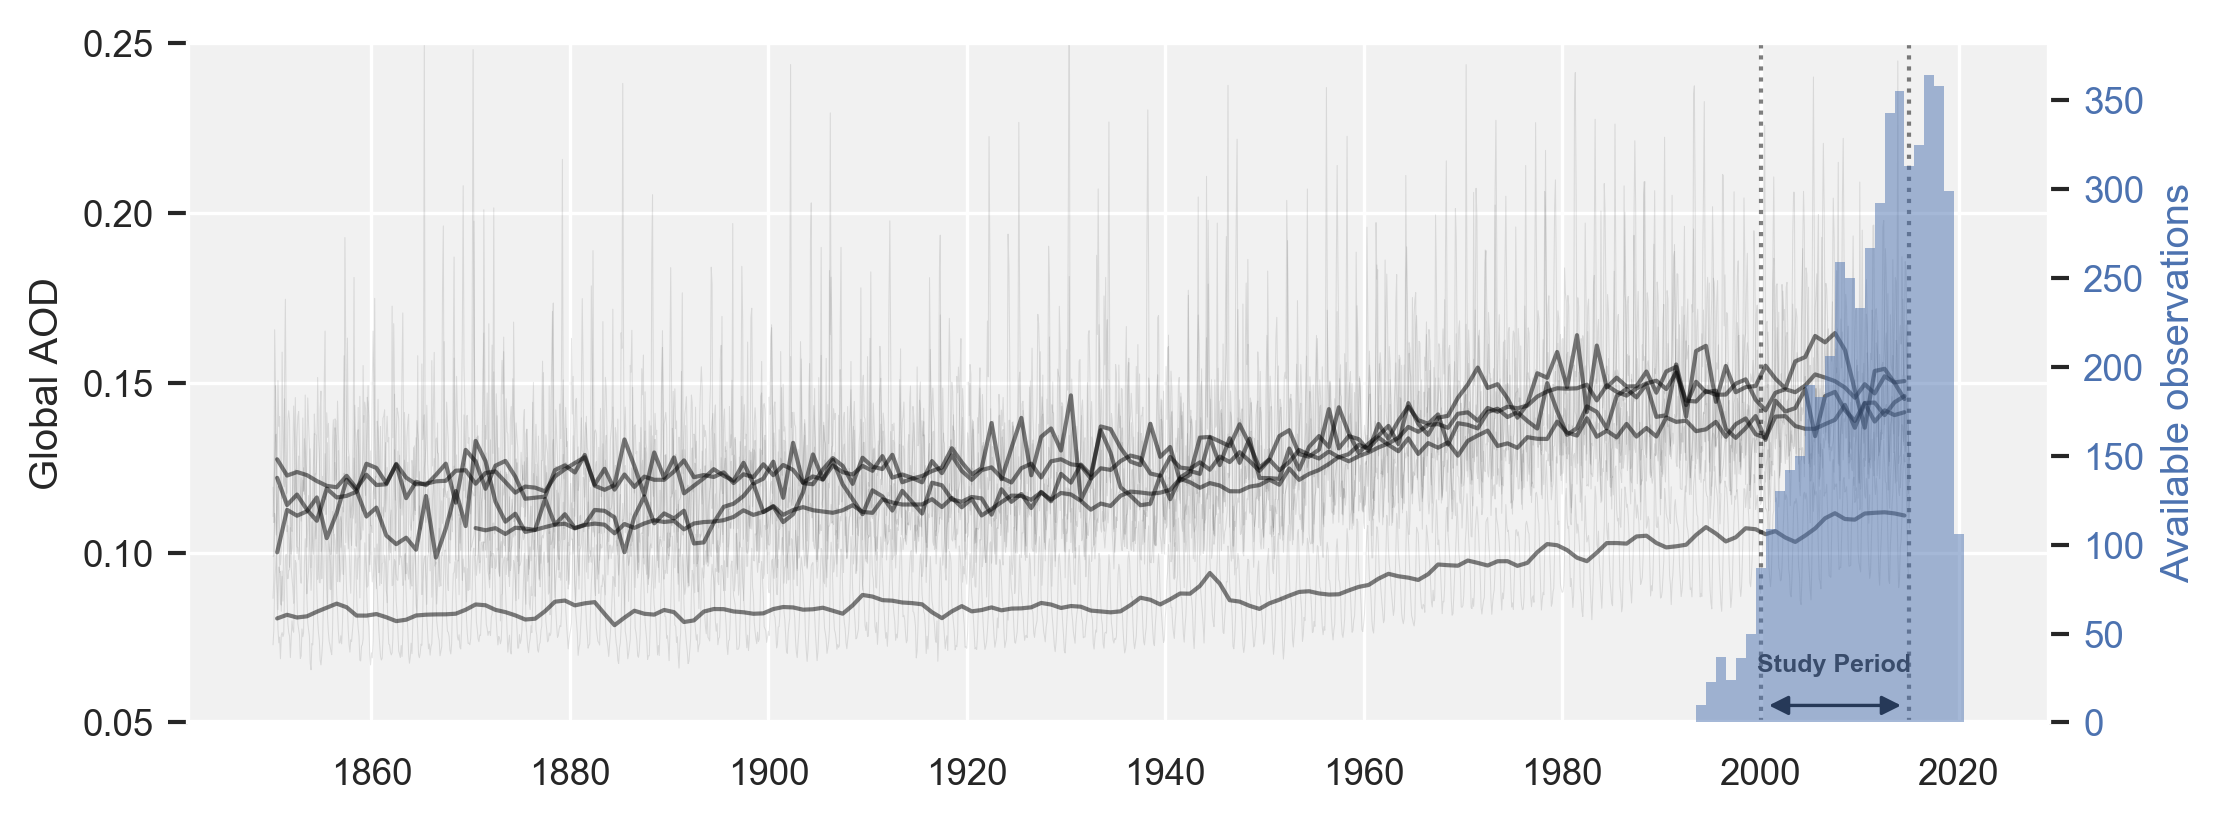
\includegraphics[width=12cm]{../scripts/figs/hist_runs.png}
 \caption{Global AOD computed from the model historical runs (black) and observations availability (blue).}
 \label{fig:hist_runs}
\end{figure}


\section{Datasets}
A set of nine column and in situ surface aerosol datasets are used in this study. The observation networks and the models providing output for these parameters are reported in Table \ref{table:datasets}.

\begin{table}
 \begin{tabularx}{\textwidth}{lllX}
  \tophline
  Parameter   & Type    & Observation network & Models                                                                                                    \\
  \middlehline
  AOD         & Column  & AERONET             & ECMWF-Rean; NorESM2; SPRINTARS; ECHAM-HAM; GEOS; OsloCTM3; GFDL-AM4; BCC-CUACE; CanESM5; CESM2; IPSL-CM6A \\
  AOD<1µm     & Column  & AERONET             & NorESM2; SPRINTARS; ECHAM-HAM; GEOS; GFDL-AM4                                                             \\
  AOD>1µm     & Column  & AERONET             & ECMWF-Rean; NorESM2; SPRINTARS; ECHAM-HAM; OsloCTM3; GFDL-AM4; BCC-CUACE                                  \\
  AE          & Column  & AERONET             & ECMWF-Rean; NorESM2; SPRINTARS; ECHAM-HAM; GEOS; OsloCTM3; GFDL-AM4                                       \\
  $PM_{2.5}$  & Surface & GAW                 & ECMWF-Rean; NorESM2                                                                                       \\
  $PM_{10}$   & Surface & GAW                 & ECMWF-Rean; NorESM2; SPRINTARS; ECHAM-HAM; GEOS                                                           \\
  $SO_{4}$    & Surface & GAW/TAD             & ECMWF-Rean; NorESM2; SPRINTARS; ECHAM-HAM; GEOS; OsloCTM3; BCC-CUACE                                      \\
  Scat. Coef. & Surface & GAW/IMPROVE/ACTRIS  & NorESM2                                                                                                   \\
  Abs. Coef.  & Surface & GAW/IMPROVE/ACTRIS  & NorESM2; SPRINTARS                                                                                        \\
  \bottomhline
 \end{tabularx}
 \caption{List of observation and model datasets used in this study.}
 \label{table:datasets}
\end{table}

\subsection{Observations}

For each of the parameters used in this study, the data of the highest quality level provided by the different observation networks were used. The mountain sites, corresponding to an elevation above 1000 m were excluded for representavity reasons (\cite{kinne2013mac}).

\subsubsection{AERONET Sun photometer}
\textcolor{red}{(AERONET website)}: The AERONET (AErosol RObotic NETwork) project is a federation of ground-based remote sensing aerosol networks established by NASA and PHOTONS (PHOtométrie pour le Traitement Opérationnel de Normalisation Satellitaire; Univ. of Lille 1, CNES, and CNRS-INSU) and is greatly expanded by networks (e.g., RIMA, AeroSpan, AEROCAN, and CARSNET) and collaborators from national agencies, institutes, universities, individual scientists, and partners. For more than 25 years, the project has provided long-term, continuous and readily accessible public domain database of aerosol optical, microphysical and radiative properties for aerosol research and characterization, validation of satellite retrievals, and synergism with other databases. The network imposes standardization of instruments, calibration, processing and distribution \cite{holben2001emerging}.

The daily files of level 2.0 (quality assured) were used for four parameters with the version 3 algorithm that provides a fully automatic cloud screening and instrument anomaly quality controls  (\cite{smirnov2000cloud,smirnov2004aeronet,giles2019advancements}). Four parameters are used in this study

\begin{itemize}
 \item Sun Direct measurements
       \begin{itemize}
        \item AOD (Aerosol Optical Depth) at 550 nm.
        \item AE (Angstrom Exponent): calculated using 440 nm and 870 nm channels.
       \end{itemize}
 \item Spectral Deconvolution Algorithm (SDA, described in \cite{o2003spectral})
       \begin{itemize}
        \item AOD<1µm (AOD for the particles whose diameter is lower than 1 µm).
        \item AOD>1µm (AOD for the particles whose diameter is greater than 1 µm).
       \end{itemize}
\end{itemize}


\subsubsection{Particulate Matter}
All the following data have been downloaded via EBAS platform (\cite{ebasweb}).
\textcolor{red}{(EBAS website)}: EBAS is a database hosting observation data of atmospheric chemical composition and physical properties. EBAS hosts data submitted by data originators in support of a number of national and international programs ranging from monitoring activities to research projects. EBAS is developed and operated by the Norwegian Institute for Air Research (NILU).

GAW \textcolor{red}{(GAW website)}: The Global Atmosphere Watch (GAW) programme of WMO is a partnership involving the Members of WMO, contributing networks and collaborating organizations and bodies which provides reliable scientific data and information on the chemical composition of the atmosphere, its natural and anthropogenic change, and helps to improve the understanding of interactions between the atmosphere, the oceans and the biosphere.
*In North America, data only until 2006*
\begin{itemize}
 \item $PM_{10}$ (\unit{µg.m^{-3}})
 \item $PM_{2.5}$ (\unit{µg.m^{-3}})
\end{itemize}

\subsubsection{$SO_{4}$ concentration}
\textcolor{red}{(trends website)}: The global dataset is prepared by the WMO/GAW Science Advisory Group for Total Atmospheric Deposition (SAG-TAD) based on data from different regional and global networks:
\begin{itemize}
 \item WMO/GAW: World Data Center for Precipitation Chemistry
 \item CASTNET: Clean Air Status and Trends Network
 \item NADP: National Atmospheric Deposition Program
 \item CAPMoN: The Canadian Air and Precipitation Monitoring Network
 \item EMEP: The European Monitoring and Evaluation Program
 \item IDAF/DEBITS: Atmospheric Chemistry Monitoring Network in Africa / DEposition of Biogeochemically Important Trace Species
 \item EANET: Acid Deposition Network in East Asia
\end{itemize}

Subset from Aas et al.
The data has been screened to be regionally representative and of satisfactory quality:
Precipitation measurements are mainly from wet-only samplers or bulk if proven comparable to wet-only.
The sampling frequency is 2 weeks or higher –mostly daily measurements, except African data where precipitation is sampled on rain events and SO2 with monthly passive samplers.
Wet deposition and volume weighted precipitation data are based on the standard rain gauge depth if that is measured in parallel. At other sites without rain gauge, the sample depth are used.
Urban sites are not included, neither sites where the surroundings have changed considerable in the period in question.
When averaging monthly data with higher sampling frequency than daily, the sample is weighted in accordance to how many days it has been sampled in that month.

\subsubsection{Optical in situ}
Due to the scarcity of stations and due to the fact that the measurements correspond to the surface level, the presence of non-representative stations, for instance stations located nearby the roads, can have large effects on the computation of the regional time series. Used level 2 data (quality controlled, hourly averaged, reported at STP) *Filtering out some of these stations. Also, use of the non-validity flags.*

\begin{itemize}
 \item (Dry) Scattering coefficient (\unit{Mm^{-1}}): from integrating nephelometers - Validity range: [-10,1000]. Excluded stations: Granada, Ispra and Monseny
 \item Absorption coefficients (\unit{Mm^{-1}}): from filter-based absorption photometers - validity range: [-1,100]. Excluded stations: Granada, Leipzig-Mitte.
\end{itemize}

\subsection{Models}
\textcolor{red}{**Describe model groups**}
A set of 11 climate models are used in this study. Their main characteristics are reported in Table \ref{table:models}. These models can be separated into three main groups.

\subsubsection{CAMS-Reanalysis}
\textcolor{red}{(ECMWF website)} The CAMS reanalysis dataset covers the period January 2003 to near real time (NRT), though currently only data for the period 2003-2018 have been released. The CAMS reanalysis is the latest global reanalysis data set of atmospheric composition (AC) produced by the Copernicus Atmosphere Monitoring Service, consisting of 3-dimensional time-consistent AC fields, including aerosols, chemical species and greenhouse gases, though GHG fields will only be released in 2019. The data set builds on the experience gained during the production of the earlier MACC reanalysis and CAMS interim reanalysis.

The CAMS reanalysis was produced using 4DVar data assimilation in CY42R1 of ECMWF’s Integrated Forecast System (IFS), with 60 hybrid sigma/pressure (model) levels in the vertical, with the top level at 0.1 hPa. Atmospheric data are available on these levels and they are also interpolated to 25 pressure, 10 potential temperature and 1 potential vorticity level(s). "Surface or single level" data are also available.

Generally, the data are available at a sub-daily and monthly frequency and consist of analyses and 48h forecasts, initialised daily from analyses at 00 UTC.

The data are archived in the ECMWF data archive (MARS) and can be retrieved using the ECMWF Public Dataset service via the WebAPI (ECMWF Member State users can access the data using MARS directly, in the usual manner).

The IFS model and data assimilation system:
The 4DVar data assimilation uses 12 hour assimilation windows from 09 UTC to 21 UTC and 21 UTC to 09 UTC.

The IFS model documentation for various model cycles can be found on https://www.ecmwf.int/en/forecasts/documentation-and-support/changes-ecmwf-model/ifs-documentation. The model used in the CAMS reanalysis includes several updates to the aerosol and chemistry modules on top of the standard CY42R1 release, which are listed below. Please note that 42r1 documentation is not available on the page, but the code for the earlier and later cycles is available for reference.

\subsubsection{AeroCom phase III}
\textcolor{red}{(Aerocom website)} Aerocom initiative The AEROCOM-project is an open international initiative of scientists interested in the advancement of the understanding of the global aerosol and its impact on climate. A large number of observations (including MODIS, POLDER, MISR, AVHHR, SEAWIFS, TOMS, AERONET and surface concentrations) and results from more than 14 global models have been assembled to document and compare state of the art modeling of the global aerosol. A common protocol has been established and models are asked to make use of the AEROCOM emission inventories for the year 2000 and preindustrial times.

\textcolor{red}{(Aerocom website - Historical Exp.)} The main aim of the historical experiment is to understand regional trends in aerosol distribution from 1850 to 2015 and make an AeroCom reference aerosol distribution dataset (1850-2015). This experiment will also quantify the aerosol impact on TOA and surface forcing with a main emphasis on the direct aerosol effect. We underscore that the CMIP6 CEDS emissions must be used for the historical simulations. Simulations can either be performed with fixed sea-surface temperature (SSTs), historically evolving SSTs or fixed meteorology for one year. We encourage radiative forcing simulations, but if difficult to achieve on a short time frame we are interested also to have the aerosol fields without forcing diagnostics. To perform radiative forcing calculation in the case of using SST fields, we encourage double radiation calls. This output should as a minimum be every 10th year until 1980, thereafter a minimum of every 5th year 1980-2015 (preference yearly).

required output:... + additional output for some models, which permits to cover the nine aerosol parameters.
Also, nudged / not-nudged AP3?

\subsubsection{CMIP6}
\textcolor{red}{(to be done)}
The upcoming 2024 IPCC sixth assessment report (AR6) will feature new state-of-the-art CMIP6 (Couple Model Intercomparison Project, Phase 6) models. Models runs in higher resolution with new physical processes.

Historical simulations: od550aer time series from 1850 to 2014.


\begin{table}[]
 \begin{tabularx}{\textwidth}{llllllX}
  \toprule
  Model      & Group     & \begin{tabular}[c]{@{}l@{}}Natural \\ interactive emissions\end{tabular} & \begin{tabular}[c]{@{}l@{}}Anthropogenic \\ emissions\end{tabular} & Meteorology & \begin{tabular}[c]{@{}l@{}}LatxLon \\ (degree)\end{tabular} & References                                                          \\ \midrule
  ECMWF-Rean & CAMS-Rean & ?                          & ?                          & ?           & 1.12x1.12                  &                                                                     \\
  SPRINTARS  & AP3       & D, SS, DMS, Oceanic VOC      & $SO_{2}$, BC, OC                & N           & 0.56x0.56                  & \cite{takemura2000global,takemura2002single,takemura2005simulation} \\
  ECHAM-HAM  & AP3       & D, SS, DMS                          & $SO_{2}$, BC, OC                          & fSST           & 1.875x1.875                  &  Tegen et al. (2019); Neubauer et al. (2019)   \textcolor{red}{(to be added)}                                        \\
  GEOS       & AP3       & ?                          & ?                          & ?           & 1.00x1.00                  &                                                                     \\
  OsloCTM3   & AP3       & ?                          & ?                          & ?           & 2.25x2.25                  & \cite{lund2018concentrations,myhre2009modelled}                     \\
  GFDL-AM4   & AP3       & ?                          & ?                          & ?           & 1.00x1.25                  &                                                                     \\
  BCC-CUACE  & AP3       & D, SS, DMS                          & $SO_{2}$, BC, OC                         & F           & 2.8x2.8                  & \cite{zhang2012simulation,zhang2014application,wang2014improvement}                                                                    \\
  NorESM2    & CMIP6     & D, SS, DMS, MSA, BVOC      & C                          & F           & 1.89x2.50                  & \cite{olivieprep, selandprep, kirkevag2018production}               \\
  CanESM5    & CMIP6     & ?                          &                            & ?           & 2.77x2.81                  & \cite{gmd-12-4823-2019}                                             \\
  CESM2      & CMIP6     & ?                          & ?                          & ?           & 0.94x1.25                  &                                                                     \\
  IPSL-CM6A  & CMIP6     & ?                          & ?                          & ?           & 1.27x2.50                  &                                                                     \\ \bottomrule
 \end{tabularx}
 \caption{Information on models used in this study.
  Anthropogenic emissions (C=CMIP6-CEDS, O=other, *=CMIP6 modified)
  Interactive natural emissions (D=dust, SS=sea salt, O=biogenic organic, V=volcanic, ...?)
  Meteorology (N=nudged to analysed meteorology, S=prescribed varying meteorology, G=coupled GCM, F=Free, fSST=fixed SST/SIC monthly fields, not nudged)
 }
 \label{table:models}
\end{table}

\section{Methods}

\subsection{Regional time series}
Due to the nature of the processes involved in the emission and the deposition of aerosols, one can expect different trends in the different regions of the World. Instead of combining the trends obtained at each individual observation station in a given region, regional time series are computed by assembling directly the measurements of these stations. A first advantage of this method is that a single trend can be computed in a given region, with an associated significance and uncertainty, which is not possible to get when combining the trends together. Also, even when a station has not provided a sufficient amount of data for computing the trend at its location, the data can still contribute to the computation of the regional time series. The computation of regional time series should be performed in regions presenting similar seasonality patterns, which constraints the maximum size of the regions.

\subsubsection{Regions definition}
Seven regions are considered in this study. The definition of these regions enables restriction of the study to a limited number of geographic areas with, however, provides a global coverage when considering the ensemble of those regions. As seen in Figure \ref{fig:map_obs}, the regions do not have a similar coverage in terms of observations. North America and Europe have the highest concentrations of instruments.
\begin{itemize}
 \item AERONET is the most important network in terms of number of instruments. In this study, the data of more than 1000 sunphotometers are used over the World. The highest density of instruments is in Europe and in the central part of North America (US). The lowest densities are found in southern Africa and Australia.
 \item Particulate Matter: 212 instruments are spread mostly over Europe and North America. In North America, the PM measurements available through EBAS are only available until the year 2006.
 \item $SO_{4}$: 346 instruments mostly in North America and Europe. A few stations are also located in Asia and North Africa.
 \item Scat. Coef. and Abs. Coef.: about 50 stations are spread over North America, Europe, North Africa and Asia. Due to time coverage issues, the data up to the year 2018 were used to compute the regional time series of these two parameters.
\end{itemize}

\begin{figure}
 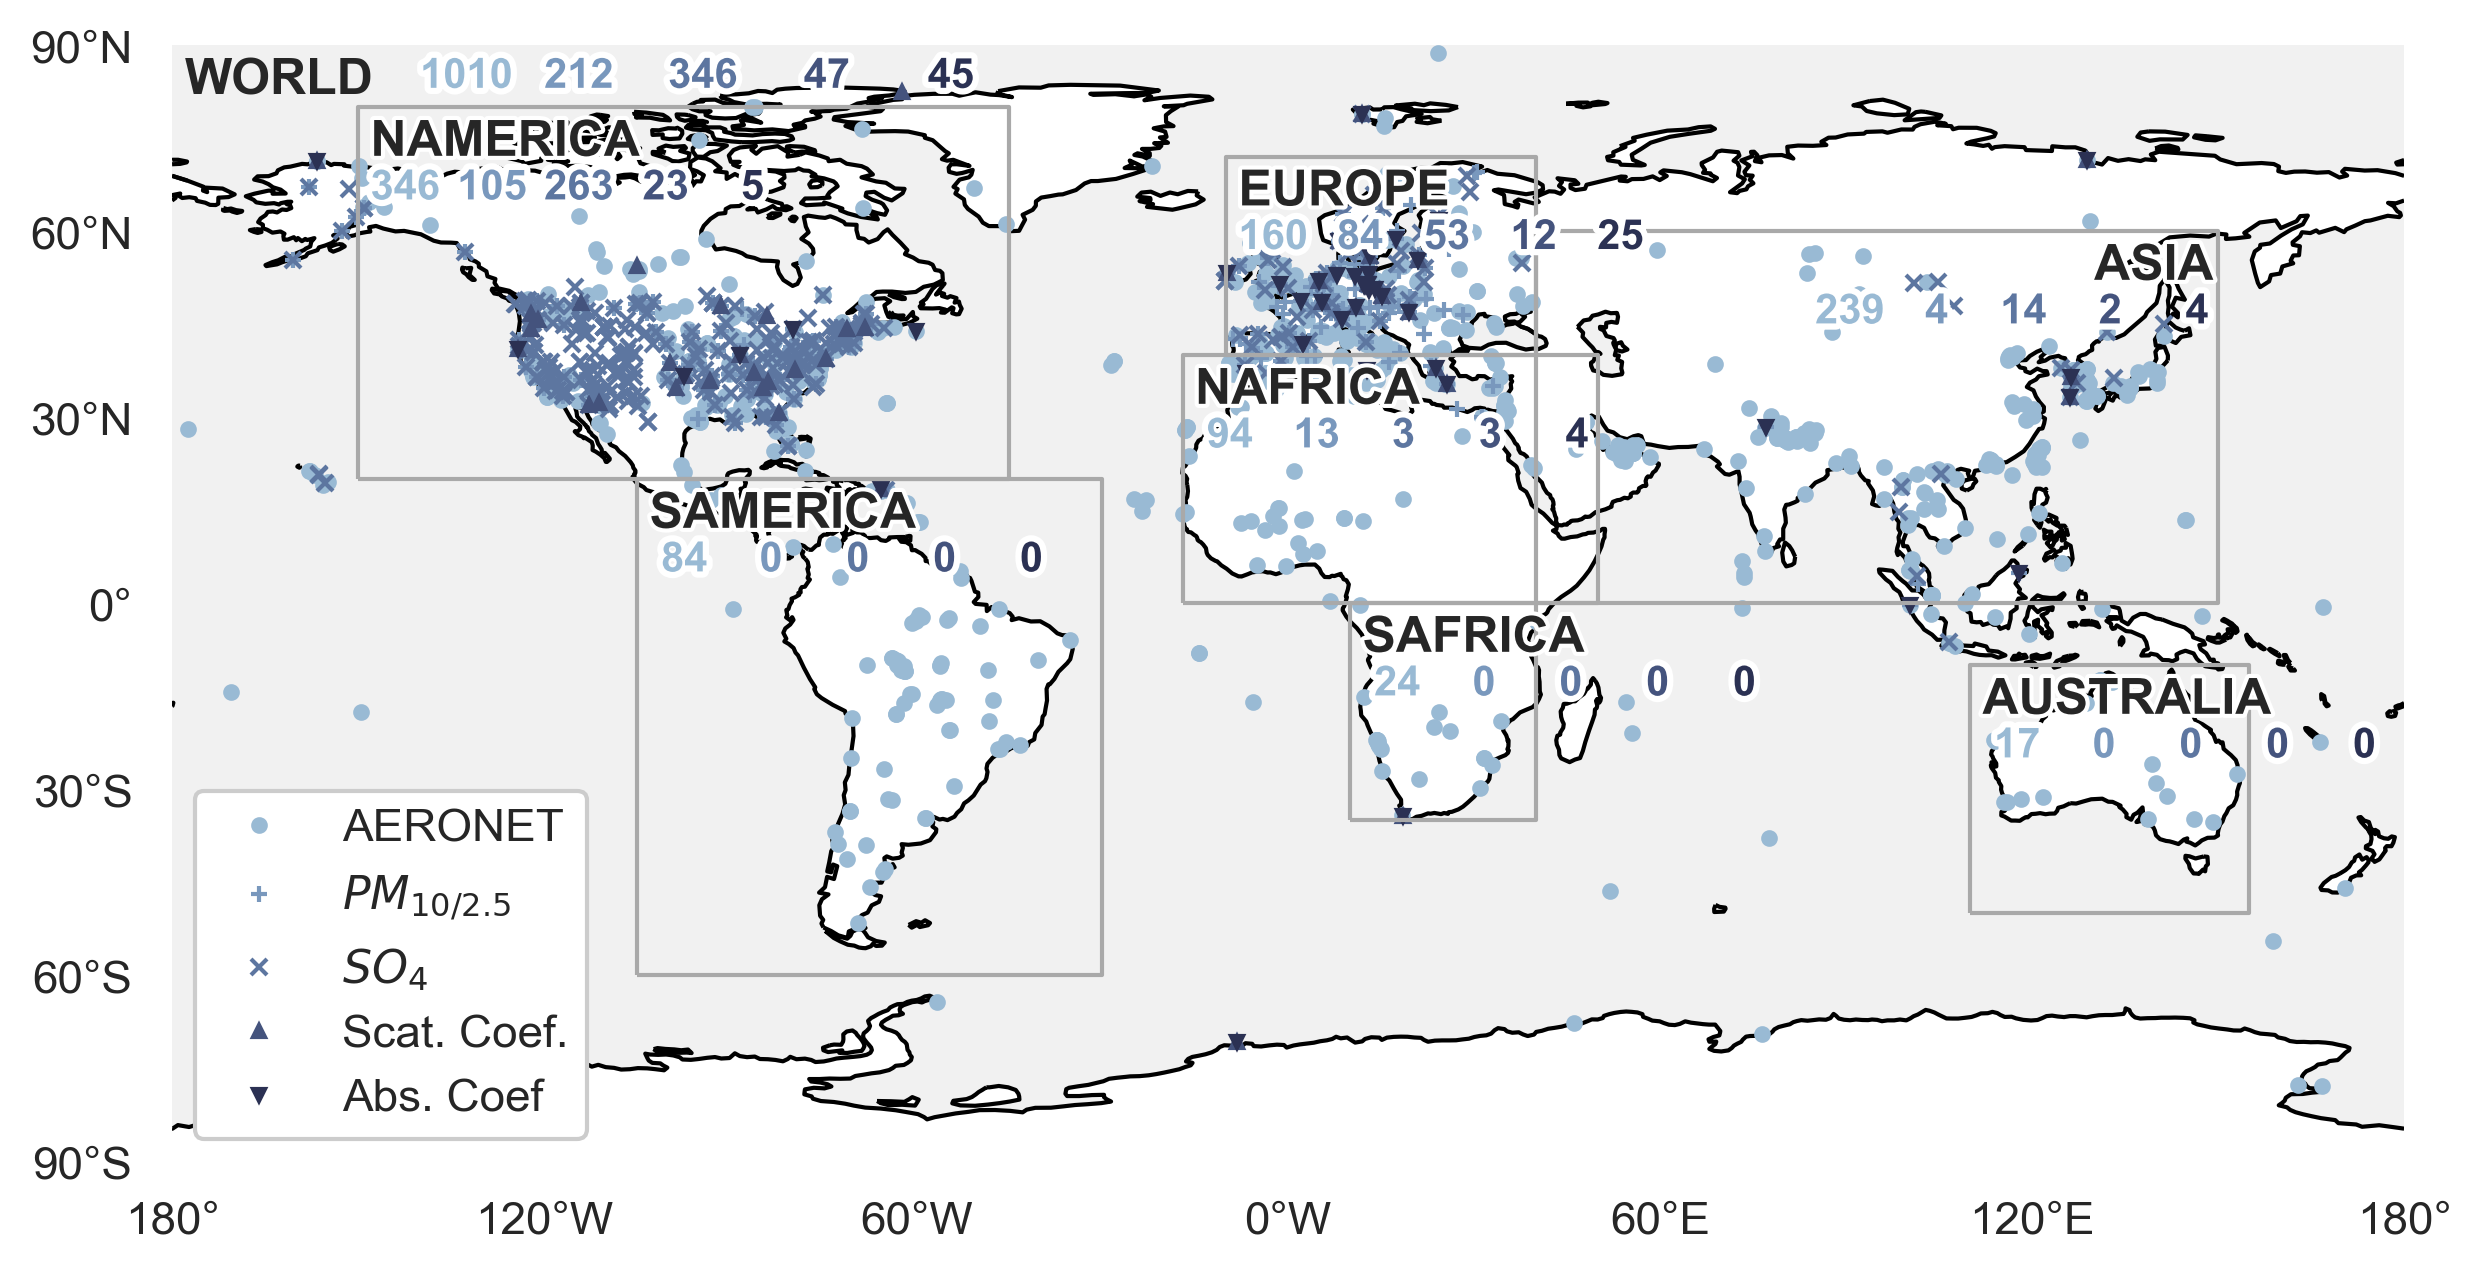
\includegraphics[width=12cm]{../scripts/figs/maps/av_obs.png}
 \caption{Observations and regions used in this study. The numbers reported within each region correspond to the maximum number of stations given for each observation network.}
 \label{fig:map_obs}
\end{figure}

\subsubsection{Constraints}
The regional time series are computed by combining, for each timestamp, the valid data of all the stations in the corresponding region. In order to construct consistent and robust regional time series, some additional data constraints are required to provide a valid point (a station with valid measurements) in the regional time series. For filtering very short term stations (e.g AERONET DRAGON stations), a minimum of 300 days with valid measurements is required for the stations that provide daily measurements. A minimum of three valid points (daily or monthly depending on the available resolution) is required per timestamp for the construction of the regional time series.

\begin{figure}
 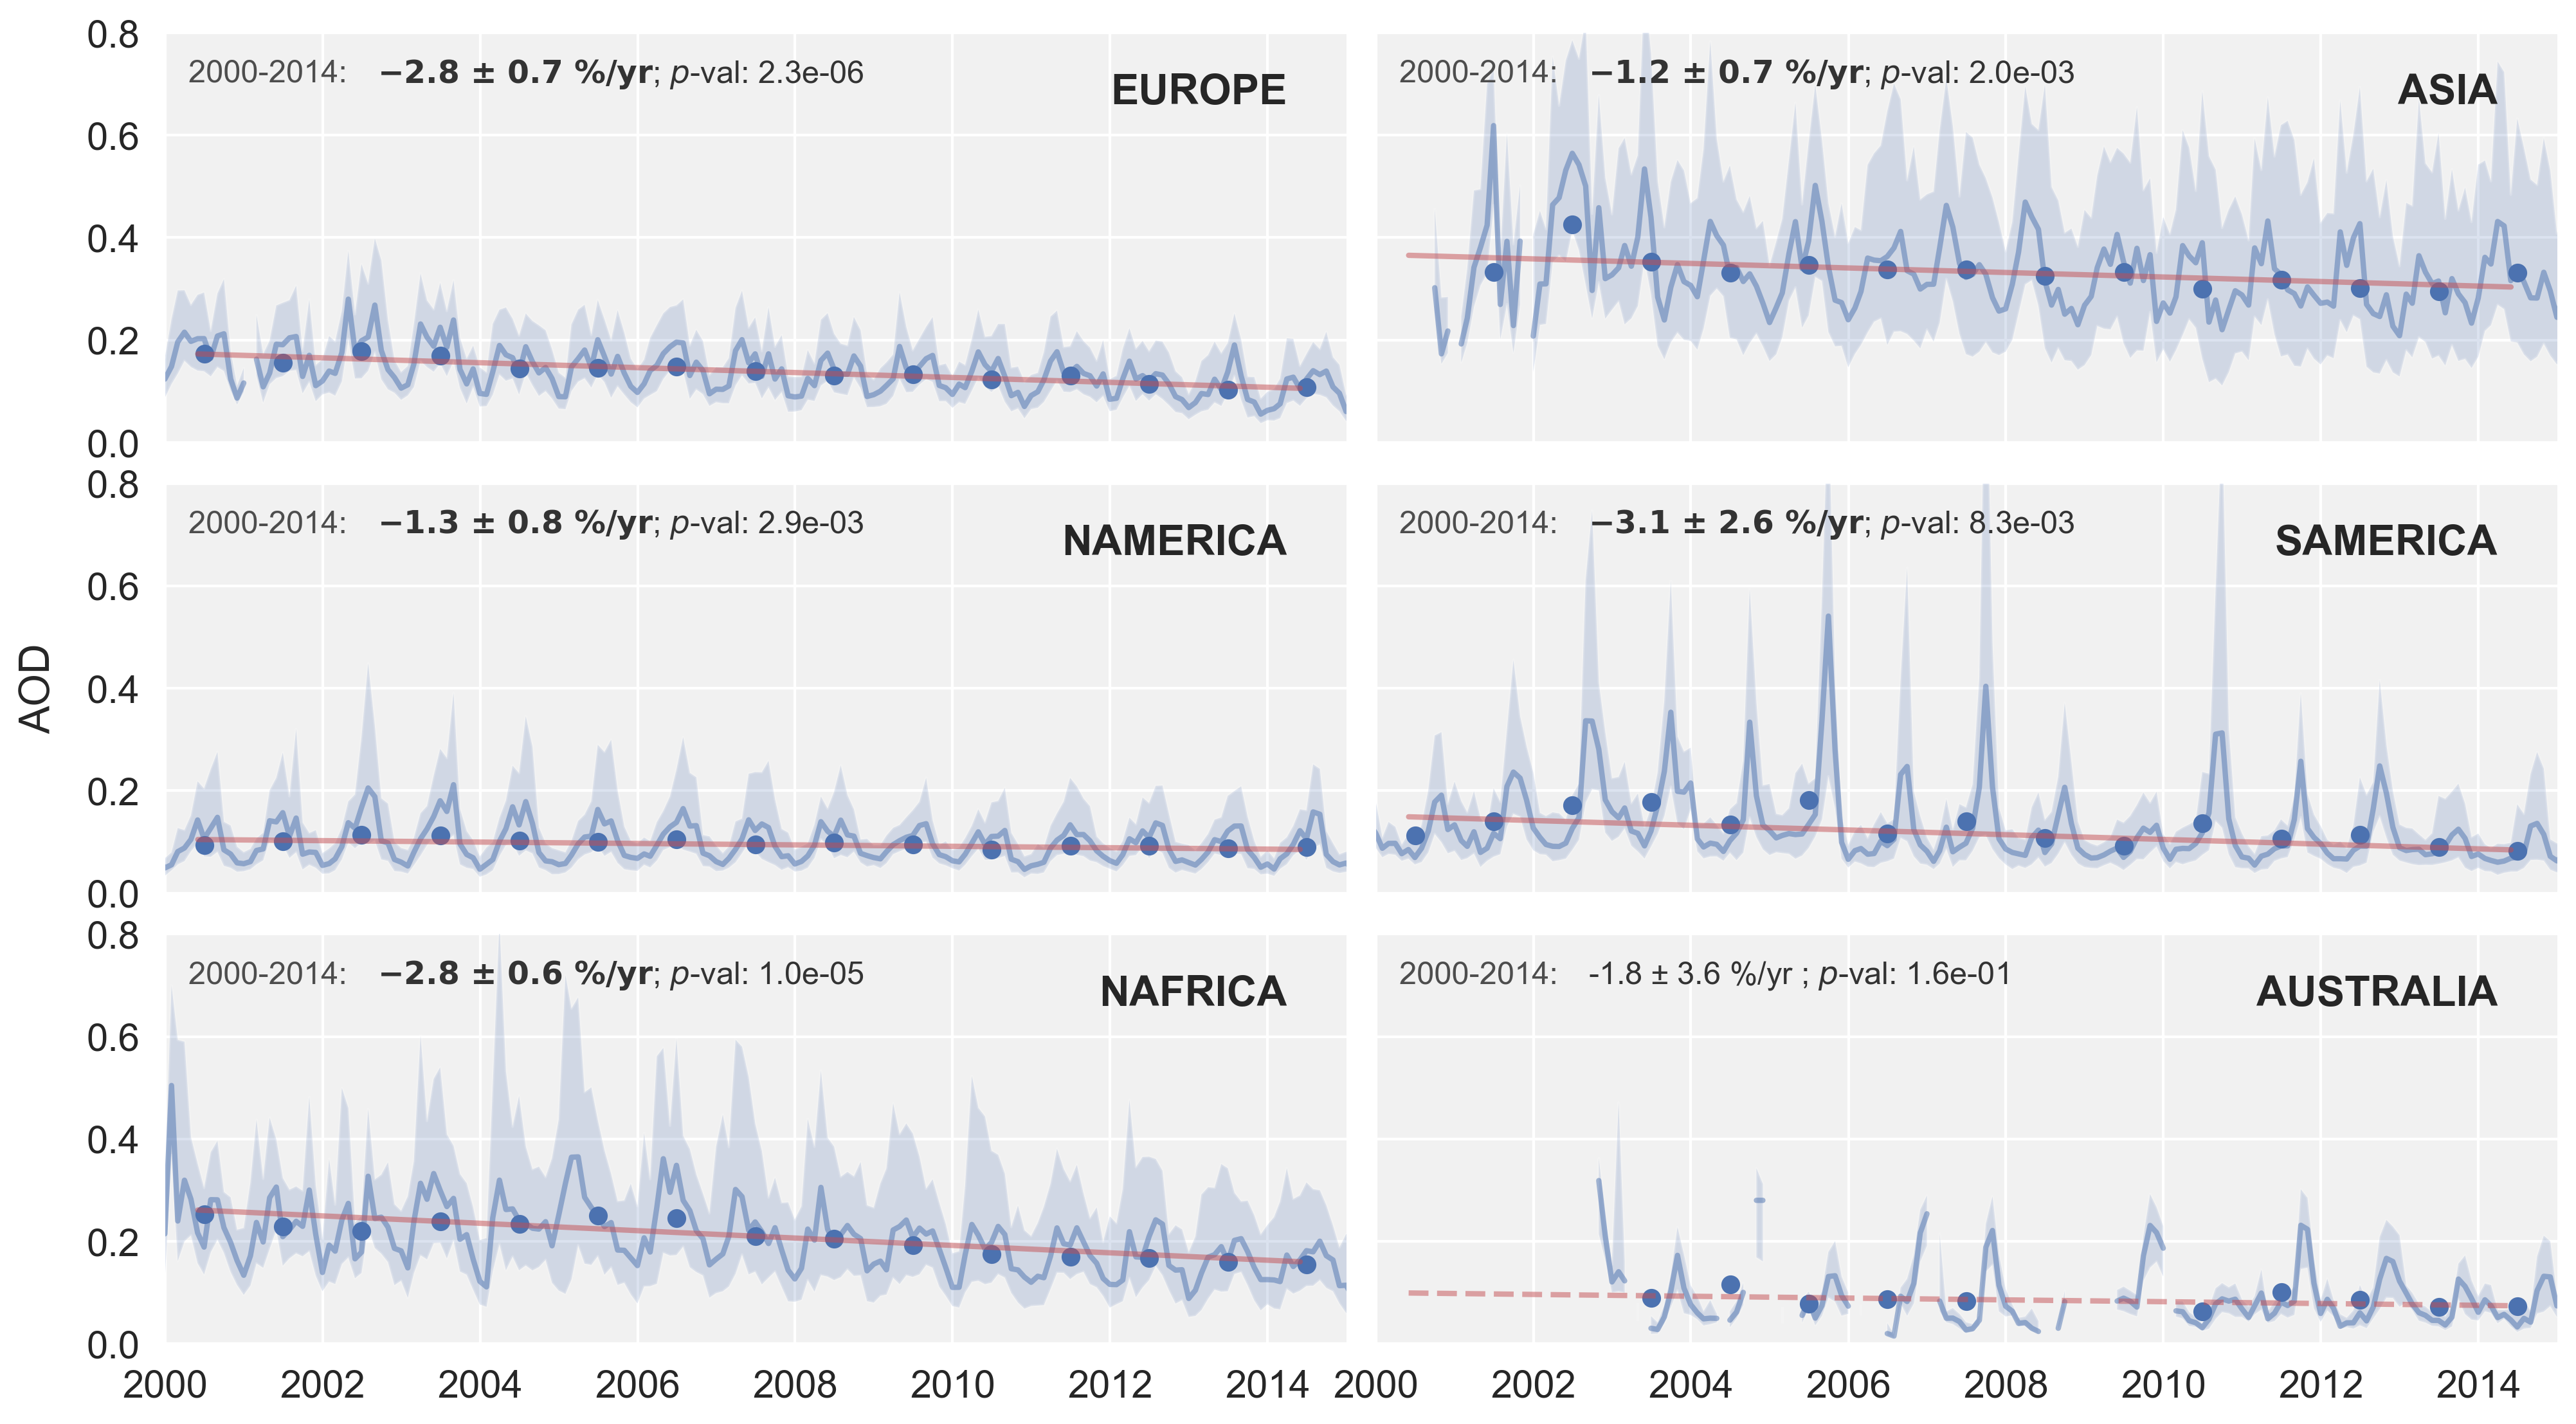
\includegraphics[width=16cm]{../scripts/figs/ts/panel-od550aer.png}
 \caption{Regional time series of AOD. The dark blue line and the light blue envelope correspond to the median and the first and third quartiles of all the valid points at the corresponding timestamp, respectively. The blue dots correspond to the yearly averages which are used to compute the linear trend, displayed as a continuous line when the trend is significant and a dashed line when it is not.}
 \label{fig:ts_aod}
\end{figure}

When those criteria are fulfilled, the median, the first and third quartiles are computed at the finest time-resolution available. The quartiles provide an indication of the inter-regional variability. An example of a regional time-series is shown in Figure \ref{fig:ts_aod} for AOD.


\subsection{Trends calculation}

\subsubsection{Regional time series computation}
The trends are computed based on the yearly averages of the regional time series. Using the yearly averages eliminates any issues caused by the seasonal cycles (observed for most of the aerosol parameters used in this study) during the calculation of the trend slope. In order to insure the statistical robustness of these yearly averages, the time averaging is performed step-by-step with specific time constraints. By starting at the finest time resolution available in the data, monthly, seasonal and yearly averages are computed when the following criteria are fulfilled:
\begin{itemize}
 \item at least 5 days per month (when daily observations are available).
 \item at least 1 month per season.
 \item at least 4 seasons per year.
\end{itemize}
These temporal constraints offer a reasonable compromise between the availability and the robustness of the yearly statistics.

\subsubsection{Trends computation}
The same methodology as described by \cite{aas2019global} was used to derive the trends of the regional time series. The significance of the trends is tested with the Mann-Kendall test. The related p-value is used to determine if the trend is significant or not within a confidence interval of 95\%. The slope is calculated with the Theil-Sen estimator which is less sensitive to outliers than standard least-squares methods. At least least 7 valid yearly averages (50\% of time coverage) are required in the regional time series for the computation of the slope.

An uncertainty is provided for each trend by combining the error of the slope calculation itself to the error of the residuals:

\begin{equation}
 Uncertainty = \sqrt{{\left (\frac{\Delta m}{y(2000)}\right )}^{2} + {\left ( \frac{m \cdot \Delta r}{y(2000)^2}\right )}^{2} }
\end{equation}

where $\Delta m$ is the Theil-Sen estimator 95\% confidence interval, $y(2000)$ is the value of the regression line at the year 2000, $m$ is the value of the Theil-Sen slope and $\Delta r$ is the averaged error on the residuals.

The trend is provided as a relative trend (\%/yr) with respect to the first year of the time period (2000).

\subsection{Representativity of the trends}
The number of available points used to compute the regional time series is not constant in time. For a given observation station, the number of points available might vary in time due to the nature of the measurements itself. For instance, classic sun photometers only measure in the daytime. Due to seasonal daylight and cloud condition variations, clear seasonal cycles are observed in the number of observations of AOD . The density of the different observation networks can also change with time. The early development of the different observation networks usually coincided with an increase in the number of observation stations. More recently, primarily for funding reasons, some networks have reduced the number of stations. This variation in the number of available measurements raises the question of time representativity for the computation of the trends.

Associated with this time representativity issue comes the space representativity issue. The data coverage is uneven across the different regions. Moreover, within a single region, the observation stations might be located in contrasting environments. Stations located in environments that are more urban, or rural, or mostly affected by natural particles, might have trends differing from the trend associated with the whole region.

Some studies have focused on the representativity of the observation stations by investigating the biases of different optical properties (\cite{wang2017,schutgens2017spatio,schutgens2019site}). This analysis is dedicated to the  representativity of the observation networks specifically for the computation of the trends. These two issues might give different results, since a stations associated with a bias, could still have a representative tendency. In order to evaluate the effect of the partial space and time sampling of the observations for the evaluation of the trends, two sensitivity studies, focusing on the time sampling and the space sampling, have been conducted using model subsets of data. For each of these studies, the trends are computed for one reference ($Ref$) and one experiment ($Exp$) dataset, and compared with each other.
\begin{itemize}
 \item Time representativity study
       \begin{itemize}
        \item $Ref_{time}$: Collocation in space and time
        \item $Exp_{time}$: Collocation in space using complete time-series
       \end{itemize}
 \item Space representativity study
       \begin{itemize}
        \item $Ref_{space}$: Collocation in space using complete time-series (=$Exp_{time}$)
        \item $Exp_{space}$: All grid-points in region using full time-series
       \end{itemize}
\end{itemize}

The difference between the relative trends are computed for each parameter and region. Those differences are then converted into a score (\unit{\%}) by using a normal distribution $f$ described by a mean $\mu=0$ and a standard deviation of $\sigma=0.5$. The choice of these parameters leads to a representativity score of 100\% when there is no difference in the trends of a reference and an experiment dataset, while a difference of 0.5\%/yr would indicates a representativity score of 50\%.

For a given parameter $p$ and a region $r$, the Representativity $Rep(p,r)$ is calculated as following

\begin{equation}
 Rep_{space,time}(p, r) = {f\left(\left| \tilde{t}_{Exp_{space,time}(p, r)}-\tilde{t}_{Ref_{space,time}(p, r)} \right|\right)}
\end{equation}
where $\tilde{t}$ is the relative trend of the corresponding dataset.

Finally, the total score is computed as the mean of the time and the space representativities. This parameter provides a

\begin{figure}[t]
 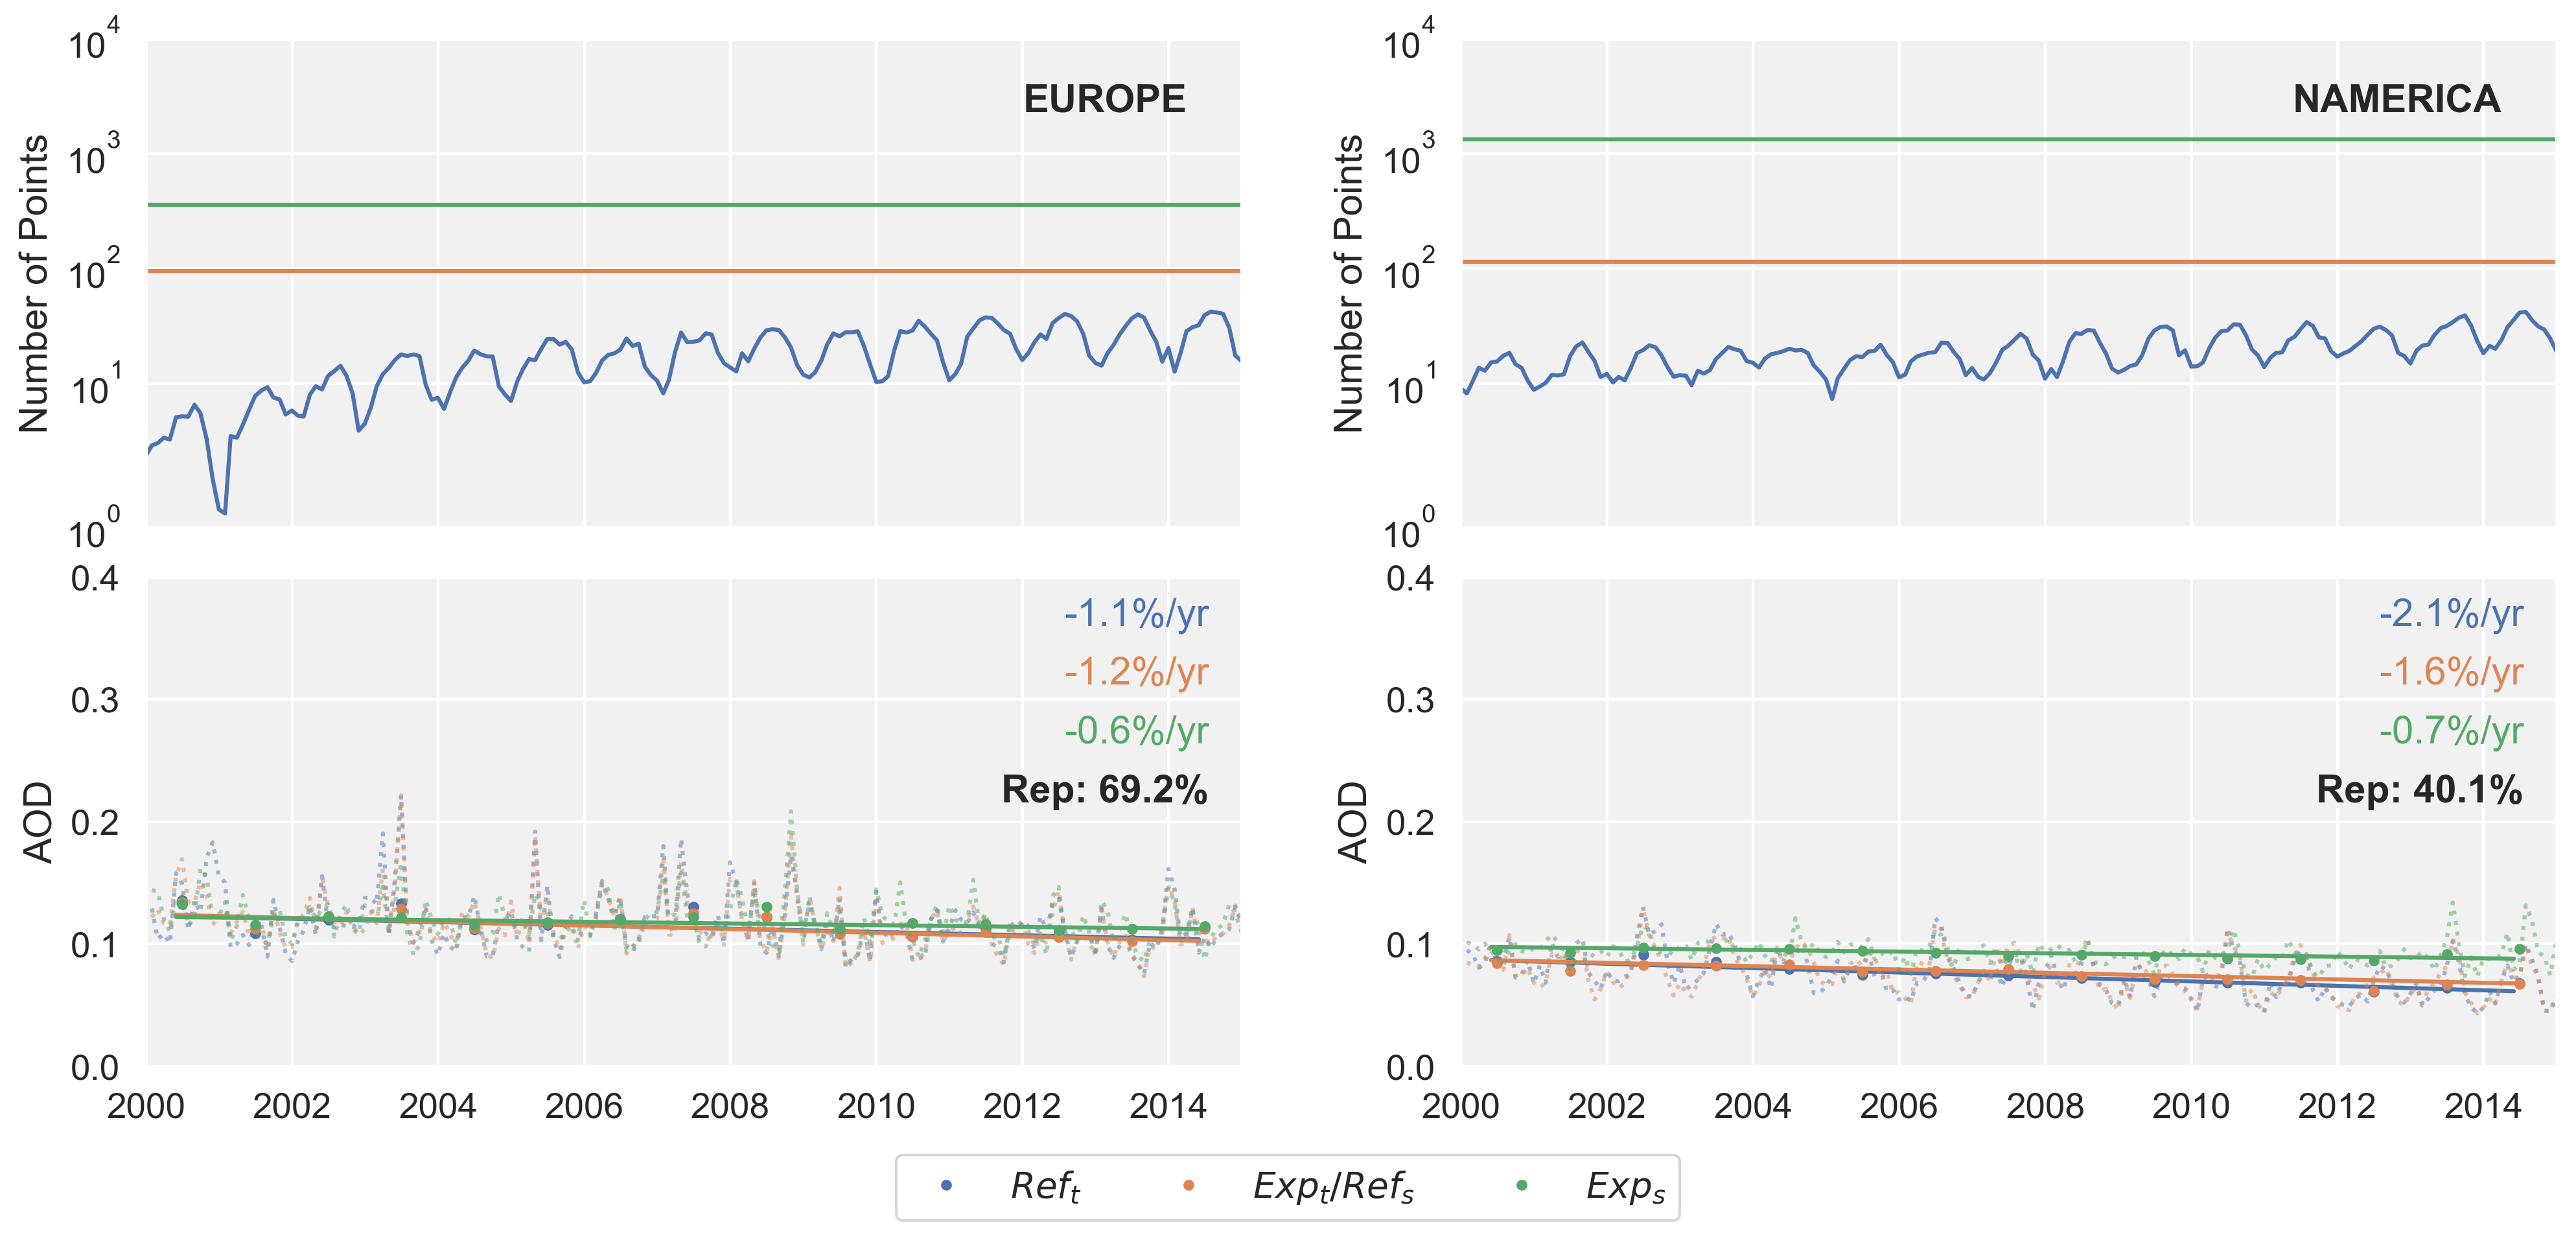
\includegraphics[width=16cm]{../scripts/figs/representativity-od550aer.png}
 \caption{Representativity of the regional AOD time series for the computation of trends assessed with model data. The upper figures correspond to the number of points used to compute the regional time series for the three different datasets. The lower figures show the time series, the trends, and the resulting representativity. $Ref_{time}$ corresponds to the model output colocated in space and time to the available observations. $Exp_{time}/Ref_{space}$ corresponds to the model output colocated in space to the stations providing measurements, using complete time series from 2000 to 2014. $Exp_{space}$ corresponds to the model output in the region without any colocation to the observations (using all gridpoints in the region).}
 \label{fig:representativity}
\end{figure}

An example of the calculation is presented in \ref{fig:representativity} for AOD in Europe and North America. In both regions, the $Ref_{time}$ dataset, corresponding to the available observations, reveals strong seasonal cycles when considering the number of points used to compute the regional time-series. These cycles are observed with most of the sun photometer datasets since the instruments only operate during daytime and cloud free conditions, and the amount of daylight and clouds varies with the season. Together with this seasonal cycle, one observes an increase in the number of points with time, which reflects the increasing number of stations over these two regions. The trends in Europe shows similar values for the time study, which means that the trend is not greatly affected by the variation of the available measurements in time. The difference is larger when considering all the grid-boxes of the domain, but the overall difference of the two studies corresponds to a representativity of 69\%. In North America, the differences in the trends between the different data sets are larger, especially for the space study. This means that the trend obtained in the whole region is significantly different from the trend obtained when considering only the grid points where observation stations are located. It should however be mentioned that the ocean grid-points are not filtered out when computing the trends over the whole domain. For this reason, the regions containing a greater proportion of ocean grid-points, where the trends are most likely to differ from those observed over land, will tend to have a lower spatial representativity. \textcolor{red}{Has this been tested? Do the trends when only land-points are taken using the full data agree with the ones that are space and time colocated?} 

This representativity study illustrates that the partial coverage in time and space of the observations leads, in some cases, to artificial trends. The representativity scores are discussed for each parameter in the following section together with the trends results.

\section{Results}

\subsection{Trends in observations}
This sections presents the trends in the observations computed for the different parameters and over the predefined regions.

\begin{table}
 \begin{tabular}{lllllll}
  \tophline
                     & EUROPE & NAMERICA & SAMERICA & NAFRICA & ASIA & AUSTRALIA \\
  \middlehline
  AOD                & 0.17   & 0.10     & 0.15     & 0.26    & 0.35 & 0.10      \\
  AOD<1µm            & 0.14   & 0.08     & 0.12     & 0.11    & 0.18 & 0.05      \\
  AOD>1µm            & 0.03   & 0.02     & 0.03     & 0.10    & 0.11 & 0.03      \\
  AE                 & 1.44   & 1.46     & 1.30     & 0.72    & 1.06 & 0.97      \\
  PM2.5 (µg.m-3)     & 12.8   & 6.0      & -        & -       & -    & -         \\
  PM10 (µg.m-3)      & 16.8   & 11.5     & -        & 19.6    & -    & -         \\
  SO4 (µg.m-3)       & 2.01   & 1.45     & -        & 2.98    & 1.97 & -         \\
  Scat. Coef. (1/Mm) & 33.2   & 25.0     & -        & -       & -    & -         \\
  Abs. Coef. (1/Mm)  & 9.7    & 2.7      & -        & -       & -    & -         \\
  \bottomhline
 \end{tabular}

 \caption{Observations means for the year 2000 (reference year used for computing the relative trends). Each value is extracted as the intercept of the linear trend computed in the 2000-2014 period for all the parameters, except for for Scat. Coef and Abs. Coef. for which the trends have been computed over 2000-2018 for time coverage reasons. One could mention that with the minimum number of yearly averages set to seven, no trend could be processed in the southern Africa region.}
 \label{table:obs_2000mean}
\end{table}

In order to compare the trends observed for the set of nine aerosol parameters in a consistent manner, we focus on the relative trends, with the reference set to the year 2000, as the first year of the study period. The means for the year 2000, reported in Table \ref{table:obs_2000mean}, reveal a great inter region variability.

The AOD is more than three times higher in Asia (AOD=0.35) than in North America and Australia (AOD=0.10). Intermediate AOD values are found in Europe and South Africa, while the second highest load is found in North Africa (AOD=0.26). In most regions, the AOD is largely dominated by its fine fraction (AOD<1µm), but this is not the case in North Africa (or Australia), where the persistent presence of desert dust makes the coarse mode (AOD>1µm) contribution to the total AOD similar in size to the fine mode contribution. This predominance of coarse particles is reflected in the AE values which exhibit lower values in North Africa (AE=0.72) and Australia (AE=0.97).

The PM observations are primarily available from Europe and North America. $PM_{10}$ observations are also available in North Africa, but the stations are mostly located in the Northern part of the region which is less affected by the dust sources than the AERONET stations in this region, which are also located in surrounding deserts. Both $PM_{10}$ and $PM_{2.5}$ are larger in Europe than in North America, with different relative proportions. In Europe, $PM_{2.5}$ represent 75\% of the $PM_{10}$, as compared to on 52\% in North America.

$SO_{4}$ means (surface mass concentrations) for the year 2000 ranges between 1.45 and 2.98 \unit{µg.m^{-3}} with the low value occurring in North America and the high value for North Africa. Similar means are found in Europe and Asia, around 2 \unit{µg.m^{-3}}.

Analogous to the surface $PM_{10}$ measurements, Scat. Coef. is higher in Europe (33.2 \unit{µg.m^{-3}}) than in North America (25.0 \unit{µg.m^{-3}}). The same feature is found for Abs. Coef. which also has higher values in Europe.

\begin{figure}[t]
 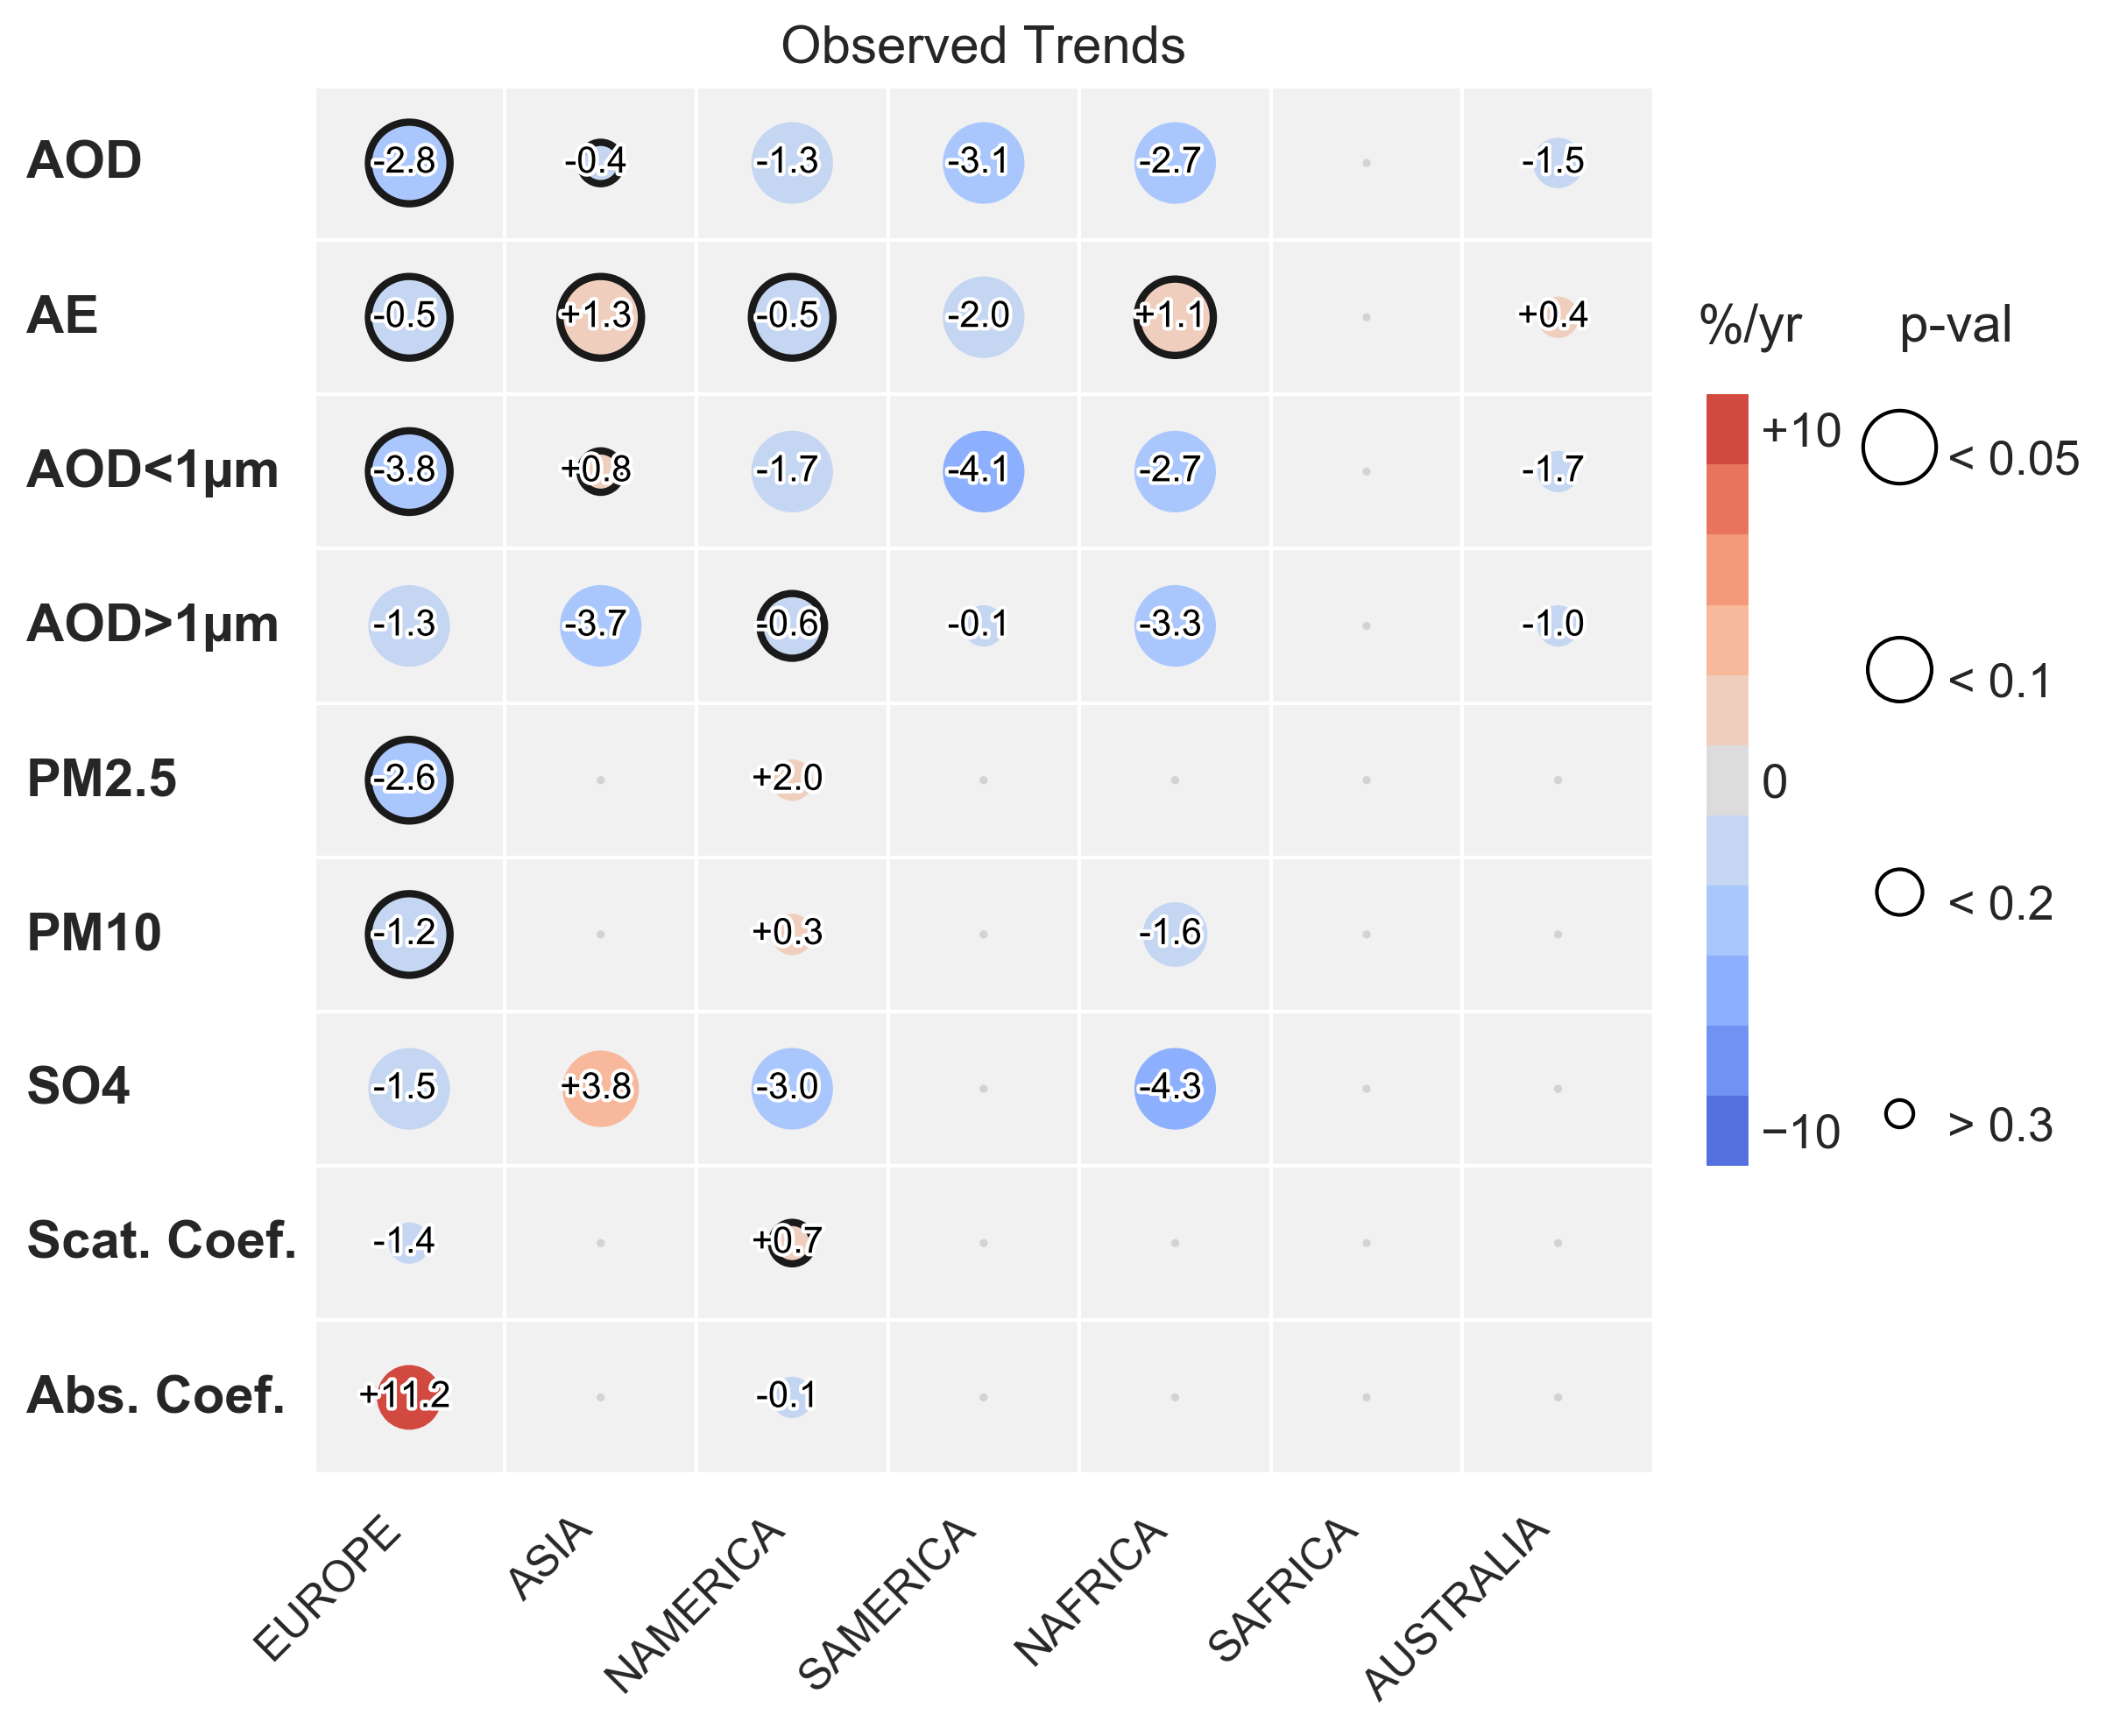
\includegraphics[width=12cm]{../scripts/figs/heatmaps/OBS.png}
 \caption{Regional trends of the aerosol properties computed with the observation datasets. The color of the circles corresponds to the slope, while the radius indicates the p-value. The largest circles represent the trends significant with a confidence of 95\%. The circles bordered with a black line indicate the trends associated with a representativity greater than 50\%.}
 \label{fig:obs_trends}
\end{figure}

The relative trends for the 2000-2014 period are shown in Figure \ref{fig:obs_trends}. The heatmap is dominated by the blue color, which indicates mostly negative trends, especially when considering the extensive parameters. Usually, the lowest p-values (<0.05) are associated with the lowest uncertainties. Each of the largest circles are then associated with a certain decrease/increase since the value of the trend is greater than the uncertainty. The uncertainties are presented in Figure \ref{fig:bars}.

\textcolor{red}{*add some comparisons with published values at individual stations?*}
\begin{itemize}
 \item In Europe, both columnar and surface parameters reveal significant decreases, with the exception of Abs. Coef. for which the observed decrease is not significant. For this last parameter, the associated uncertainty of the trend exceeds the trend itself. This large uncertainty is induced by the low data coverage in the earliest period. For the other parameters, the uncertainties are lower than the trends. A decrease in AOD (-2.8\%/yr) is found for both fine and coarse mode particles. This is consistent with the negative trends found at some individual stations in this region (\cite{glantz2019}). The fine mode is decreasing more than the coarse mode, which is consistent with the decrease observed for AE. The same pattern is found at the surface since $PM_{2.5}$ has decreased by factor of two relative to $PM_{10}$. These trends could result from the mitigation measures aiming for reduced anthropogenic aerosols emissions. This is more directly observed in the decrease of $SO_{4}$ (-1.5\%/yr). The representativity study reveals that the observed trends are actually representative for the whole period and region for all of the parameters, except for Scat. Coef. and Abs. Coef. due to the lack of observations in the earliest period. A good agreement is found with the trends obtained at individual stations and reported by \cite{collaudcoenprep}, which reports on decreases of -2.92\%/yr for Scat. Coef. and -4.2\%/yr for Abs. Coef., as compared to -2.9\%/yr and -2.1\%/yr in this study.
 \item In North America, similar trends are found for the columnar properties as were found for Europe. AOD is decreasing at a rate of 1.3\%/yr, a 55\% percent smaller trend than observed in Europe, but the North America reference value in 2000 is 40\% lower than the reference value in Europe. PM measurements are not available after 2006 within EBAS \textcolor{red}{**to be updated**}, which leads to uncertain and not significant trends. $SO_{4}$ decreases by about 3\%/yr, which is twice as large as the decrease observed in Europe, where the reference value is however larger than in North America. The sulfate trend is similar to the trend reported by \cite{aas2019global} in this region (-3.15\%/yr). The regional time series are extend farther back in time for Scat. Coef. and Abs. Coef. in North America than in Europe. However, no significant trends are found for these data sets. One can note that the representativity scores are higher for AE than for AOD, while these two parameters have the same amount of data. This means that the trends are probably smoother, in space and time, when comparing AE with AOD, which makes a same amount of available observations more representative in the first case. \cite{collaudcoenprep} finds a large decrease for Scat. Coef. (-2.57\%/yr) which is not found, in this study, when using regional time series. Similar values are found for Abs. Coef. (-1.85\%/yr) despite the fact the trend is not significant.
 \item All of the columnar properties show decreasing trends in South America. All the trends are significant, except for AOD>1µm. As shown in the regional time series in Figure~\ref{fig:ts_aod}, the observed decrease in AOD coincides with a diminution of the intensity of the seasonal peaks, happening around September. The same patterns are found for AOD<1µm. *Forest Fires? Why does it decrease?*
 \item In North Africa, while significant decreases are found for all AOD parameters, an increase of AE (+1.1\%/yr) is observed, which indicates an increase in the proportion of fine particles with time. This is consistent when considering the AOD of the fine and coarse modes, which reveal a larger decrease for AOD>1µm.
 \item AE is also increasing in Asia as a combination of a (not significant) increase in AOD<1µm and a significant increase in AOD>1µm. This result is consistent with the trend reported by \cite{yoon2012trend} at some individual stations. At the same time, we observe an increase of $SO_{4}$ of 3.8\%/yr, which is consistent with the trend reported in \cite{aas2019global}. This increase is associated with a large uncertainty ($\pm$4\%/yr ) due to a drop in the already small number of stations available in the region, especially between 2010 and 2012. Indeed, with a maximum of 12 stations, a few stations missing can greatly affect the computation of the regional time series. This is reflected by the representativity study which reveals a score lower than 40\% for this parameter. 
 \item No significant trends could be found in Australia, while the representativity is greater than 50\% for AOD, AOD<1µm and AE.

\end{itemize}

This multi-parameter trends analysis reveals a decrease in most of the extensive parameters, both in the total column and at the surface level. In Asia, the trends in AOD<1µm, AE and SO4 suggest an increase in the proportion of the finer particles. While differences might be expected when comparing regional trends with trends computed at individual stations, consistent trends are usually found with literature. With a regional approach, \cite{DEMEIJ201275} focused on the AOD trends in the 2000-2009 period. Considering the differences in the study periods, and the methodologies involved, consistent trends can be found in most of the regions.

\subsection{Evaluation of the models trends against observations}

\begin{figure}[t]
 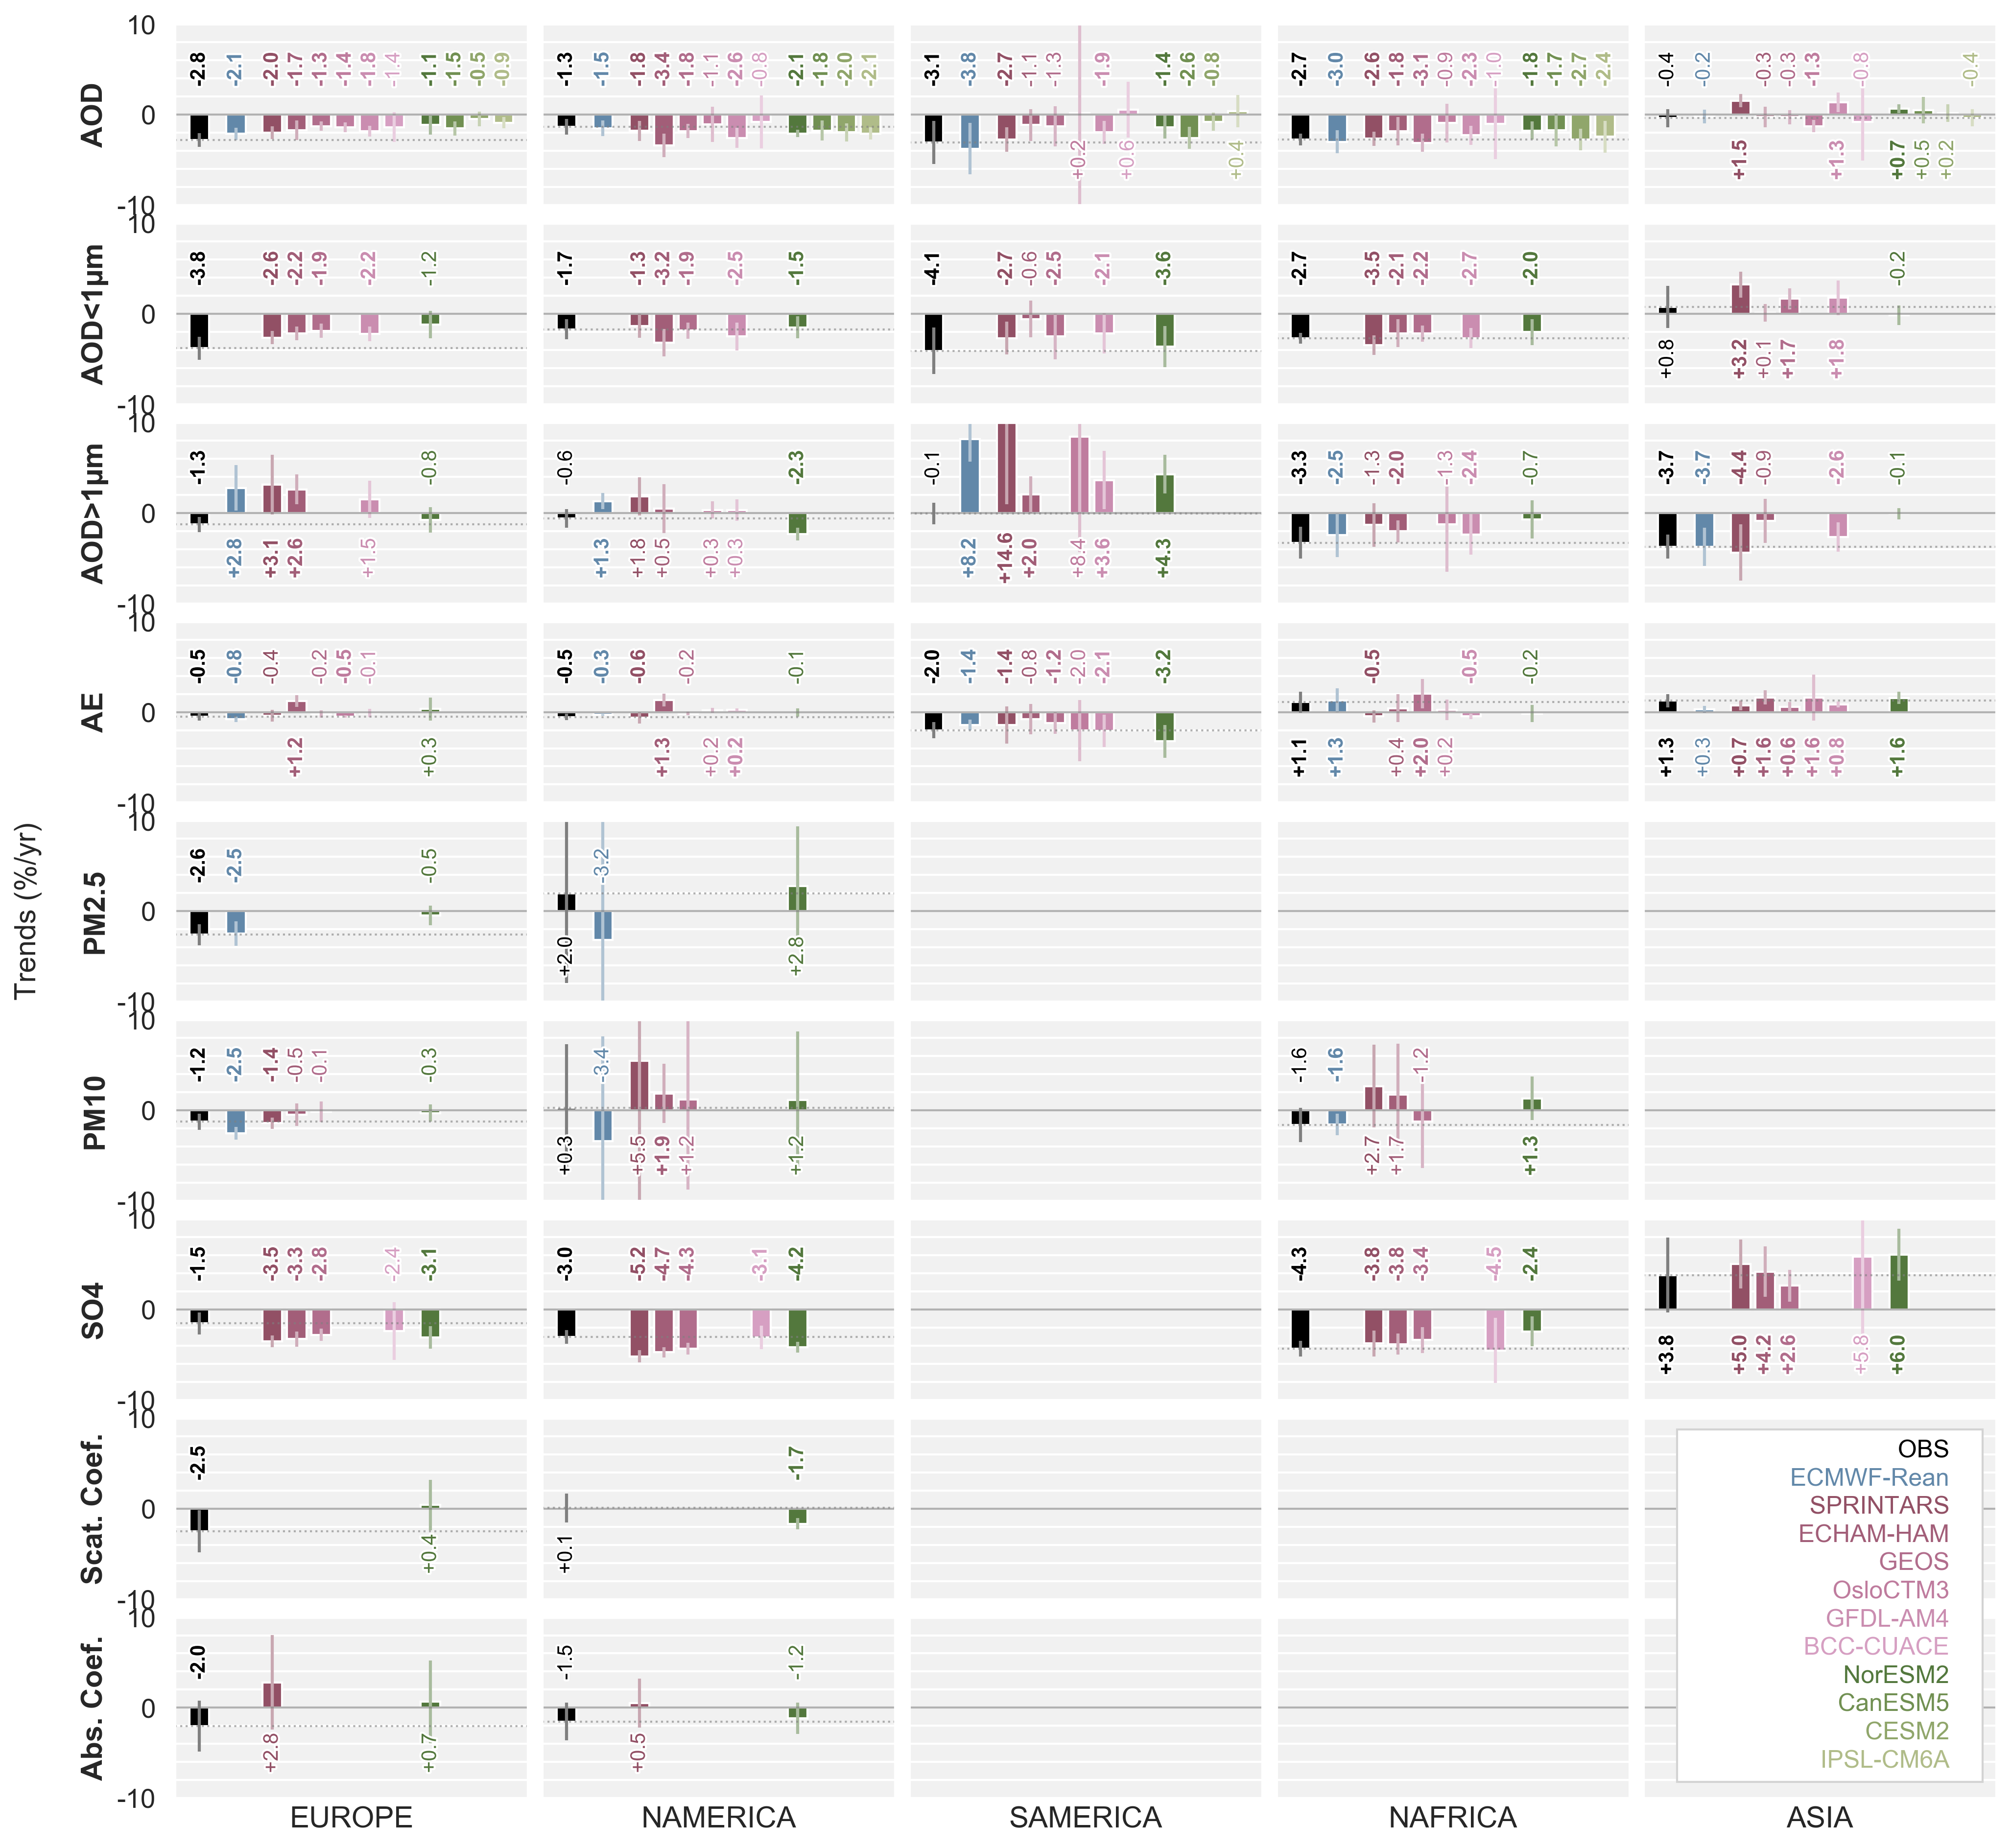
\includegraphics[width=16cm]{../scripts/figs/heatmaps/BARS.png}
 \caption{Regional trends of the aerosol properties computed with observations and models colocated in space and time to the observations. The error bars correspond to the uncertainty of the trend as calculated using both the uncertainty on the Theil−Sen slope and the residuals. The bold font indicates that the trends are significant with an expectancy of 95\% (p-val<0.05).}
 \label{fig:bars}
\end{figure}

In order to evaluate the trends from the models, the regional time series have been computed with the model output colocated in space and time to the available observations at the stations level. The trends are computed similarly as for the observation datasets. However, for the few models providing output every 5 years (in addition to 2014), the minimum number of points has been reduced from 7 to 4, so the trends can be computed using the years 2000, 2005, 2010 and 2014 *e.g: OsloCTM*. The results, shown in Figure \ref{fig:bars}, reveal different performances of the various models, for the reproduction of the observed trends, depending on the parameters and the regions.


\begin{itemize}
 \item AOD: the models show trends in the same direction as the observations over all the regions except in Asia, where the associated uncertainties are, however, usually larger than the trend values. Some differences between the three groups of models can be noticed when investigating the different regions:
       \begin{itemize}
        \item EUROPE: all the groups underestimate the observed decrease. With an average decrease of -1.0\%/yr, the CMIP6 models exhibit the highest underestimation, while the best performance is obtained with CAMS-Rean (-2.1\%/yr). The AP3 models trends range from -1.3\%/yr to -2.0\%/yr.
        \item NAMERICA: in contrast to the results for EUROPE, on average, all of the models overestimate the observed decrease in NAMERICA even though two models of the AP3 group simulate lower trends than found for observations. The consistency in the trends is very high within the CMIP6 group over this region.
        \item SAMERICA: CAMS Rean slightly overestimates the observed decrease while all the models of the two other groups underestimate this decrease. A few of them are capturing positive trends, but associated with large uncertainties.
        \item NAFRICA: all the models capture the observed decreasing tendency. With a trend of -3.0\%/yr, CAMS-Rean is closer to the observations (-2.7\%/yr). AP3 and CMIP6 multi-model averages are -2.0\%/yr and -2.2\%/yr, respectively.
        \item ASIA: A large inter-model variability is found in this region where the uncertainty is also significant. The means of the trends of each group range from -0.2\%/yr to +0.2\%/yr.
       \end{itemize}
 \item AOD<1µm: usually, the same patterns are found as for AOD. The models that underestimated the AOD are underestimating AOD<1µm and vice versa. For AOD<1µm and the following parameters, only NorESM2 provides data for the CMIP6 group.
       \begin{itemize}
        \item in EUROPE: the underestimation of the decrease captured by the models happens in a larger extent as compared to AOD.
        \item ASIA: an increase, associated to large uncertainties is found in both models of the AP3 group (+1.3\%/yr) and observations (+0.8\%/yr).
       \end{itemize}
 \item AOD>1µm: the performances of the models are not as good as for AOD<1µm *Link with Jonas paper: the performances of the models are also generally lower in the evaluation study*. The inter model variability is also higher since some models are capturing trends in opposite directions.
       \begin{itemize}
        \item EUROPE: while the observations exhibit a significant decrease, CAMS-Rean and all of the AP3 models exhibit increasing values for AOD>1µm. NorESM2 from CMIP6 simulate a decrease consistent with the observations.
        \item SAMERICA: All of the models simulate large increases, from +4.3\%/yr up to +14.6\%/yr  which are not visible in the observations (-0.1\%/yr).
        \item NAFRICA: the models reproduce the observed decrease of 3.3\%/yr to some extent (from -0.7\%/yr to -2.5\%/yr).
        \item ASIA: CAMS-Rean captures the same trend as computed with the observations dataset. Like for AOD<1µm, no certain trend can be identified  in this region with the CMIP6 model.
       \end{itemize}
 \item AE: the trends are usually relatively lower than for AOD in the respective regions. This feature is visible with both observations and models.
       \begin{itemize}
        \item EUROPE and NAMERICA: one model of the AP3 group (ECHAM-HAM) simulates a significant positive trend while negative tendencies are found in the observation and with the other models.
        \item SAMERICA: all of the models simulate negative trends, most of them significant, in agreement with the observations. CAMS-Rean and the AP3 models tend to underestimate the decrease, while the CMIP6 model tends to overestimate it.
        \item NAFRICA: CAMS-Rean reproduces well the observed increase (+1.3\%/yr VS +1.1\%/yr). The significant trends of the AP3 models range from -0.5\%/yr to +2.0\%/yr.
        \item ASIA: the AP3 models and the CMIP6 model exhibit significant positive trends, which is also the case for the observations. CAMS-Rean does not capture any significant trend in this region.
       \end{itemize}
 \item PM2.5: since no PM observation is available after the year 2006 in North America, the trends are associated with large uncertainties which makes the validation more difficult in this region. However, when discarding these uncertainties, the trends seem to be well captured by NorESM2, in contrast to CAMS-Rean, which performs well in Europe.
 \item PM10: CAMS-Rean reproduces the observed decrease in North Africa well, but overestimates the decrease in Europe. In North Africa, three of the five models available exhibit positive trends, the opposite to the trends based on observations.
 \item $SO_{4}$: The AP3 and CMIP6 models perform pretty well for the SO4 surface concentration. The magnitude of the model trends is however higher than the observed trends in all the regions except North Africa.
 \item Scat. Coef. and Abs. Coef.:  as mentioned in the previous section, the observations trends have been computed for these two parameters using data until 2018. The two models providing output for these parameters are NorESM2 and SPRINTARS. The first model provides data until 2014, so the trends correspond to the period [2000-2014], while the second one provides data until 2018 and then covers the whole observation period [2000-2018].
       \begin{itemize}
        \item EUROPE: a significant decrease is found in Scat. Coef. observations, which is captured by NorESM2 in a lower extent. For Abs. Coef., the uncertainty of the trend is larger than the value of the trend, but the model trends exhibit opposite signs to the observed trends.
        \item NAMERICA: A significant decrease is found with NorESM2 for Scat. Coef. which is not seen in the observations. For Abs. Coef, NorESM2 captures a similar trend as derived from the observations, while SPRINTARS does not.
       \end{itemize}
\end{itemize}

This model trends evaluation reveals some key-points. Firstly, CAMS-Rean, which assimilates AOD, performs the best for capturing the trends of this parameter. Second, a large inter-model variability is generally found over Asia, where the observed trends are also the most uncertain.
Considering the total column, the models usually perform rather well for AOD, AOD<1µm, and AE, but show lower skill for AOD>1µm. At ground level, the models perform well for SO4 concentration, and Scat. Coef in despite of the larger uncertainties due to both observation and models data amount. There is a quite large inter-model variability for the PM trends. \textcolor{red}{what about absorption?}

**Can we identify significant differences between the model groups and link that to Table \ref{table:models}??**

\subsection{Trends in models}

\subsubsection{Global trends}

\begin{table}
 \begin{tabular}{lll}
  \tophline
                                & $Mean_{2000}$ & Trend (\%/yr) \\
  \middlehline
  AOD                           & (0.16) 0.14   & (+0.1) +0.2   \\
  AOD<1µm                       & (0.09) 0.05   & (+0.4) +0.6   \\
  AOD>1µm                       & (0.06) 0.09   & (-0.2) +0.1   \\
  AE                            & (0.78) 0.43   & (+0.2) +0.3   \\
  $PM_{2.5}$ (\unit{µg.m^{-3}}) & (12.4) 9.1    & (+0.2) +0.2   \\
  $PM_{10}$ (\unit{µg.m^{-3}})  & (19.3) 18.7   & (+0.1) +0.1   \\
  $SO_{4}$ (\unit{µg.m^{-3}})   & (2.33) 0.64   & (-1.1) +0.4   \\
  Scat. Coef. (\unit{Mm^{-1}})  & (28.0) 21.2   & (+0.3) +0.2   \\
  Abs. Coef. (\unit{Mm^{-1}})   & (3.1) 0.9     & (+1.8) +1.5   \\
  \bottomhline
 \end{tabular}
 \caption{Global means and trends of aerosol parameters using NorESM2 data. The value in parenthesis is obtained by aggregating only grid-points where observation stations are located while using the complete model time series. The relative trends are calculated by averaging the absolute trends within the considered grid-points and normalizing it to the global mean for the year 2000.}
 \label{table:global_trends}
\end{table}

\begin{figure}[t]
 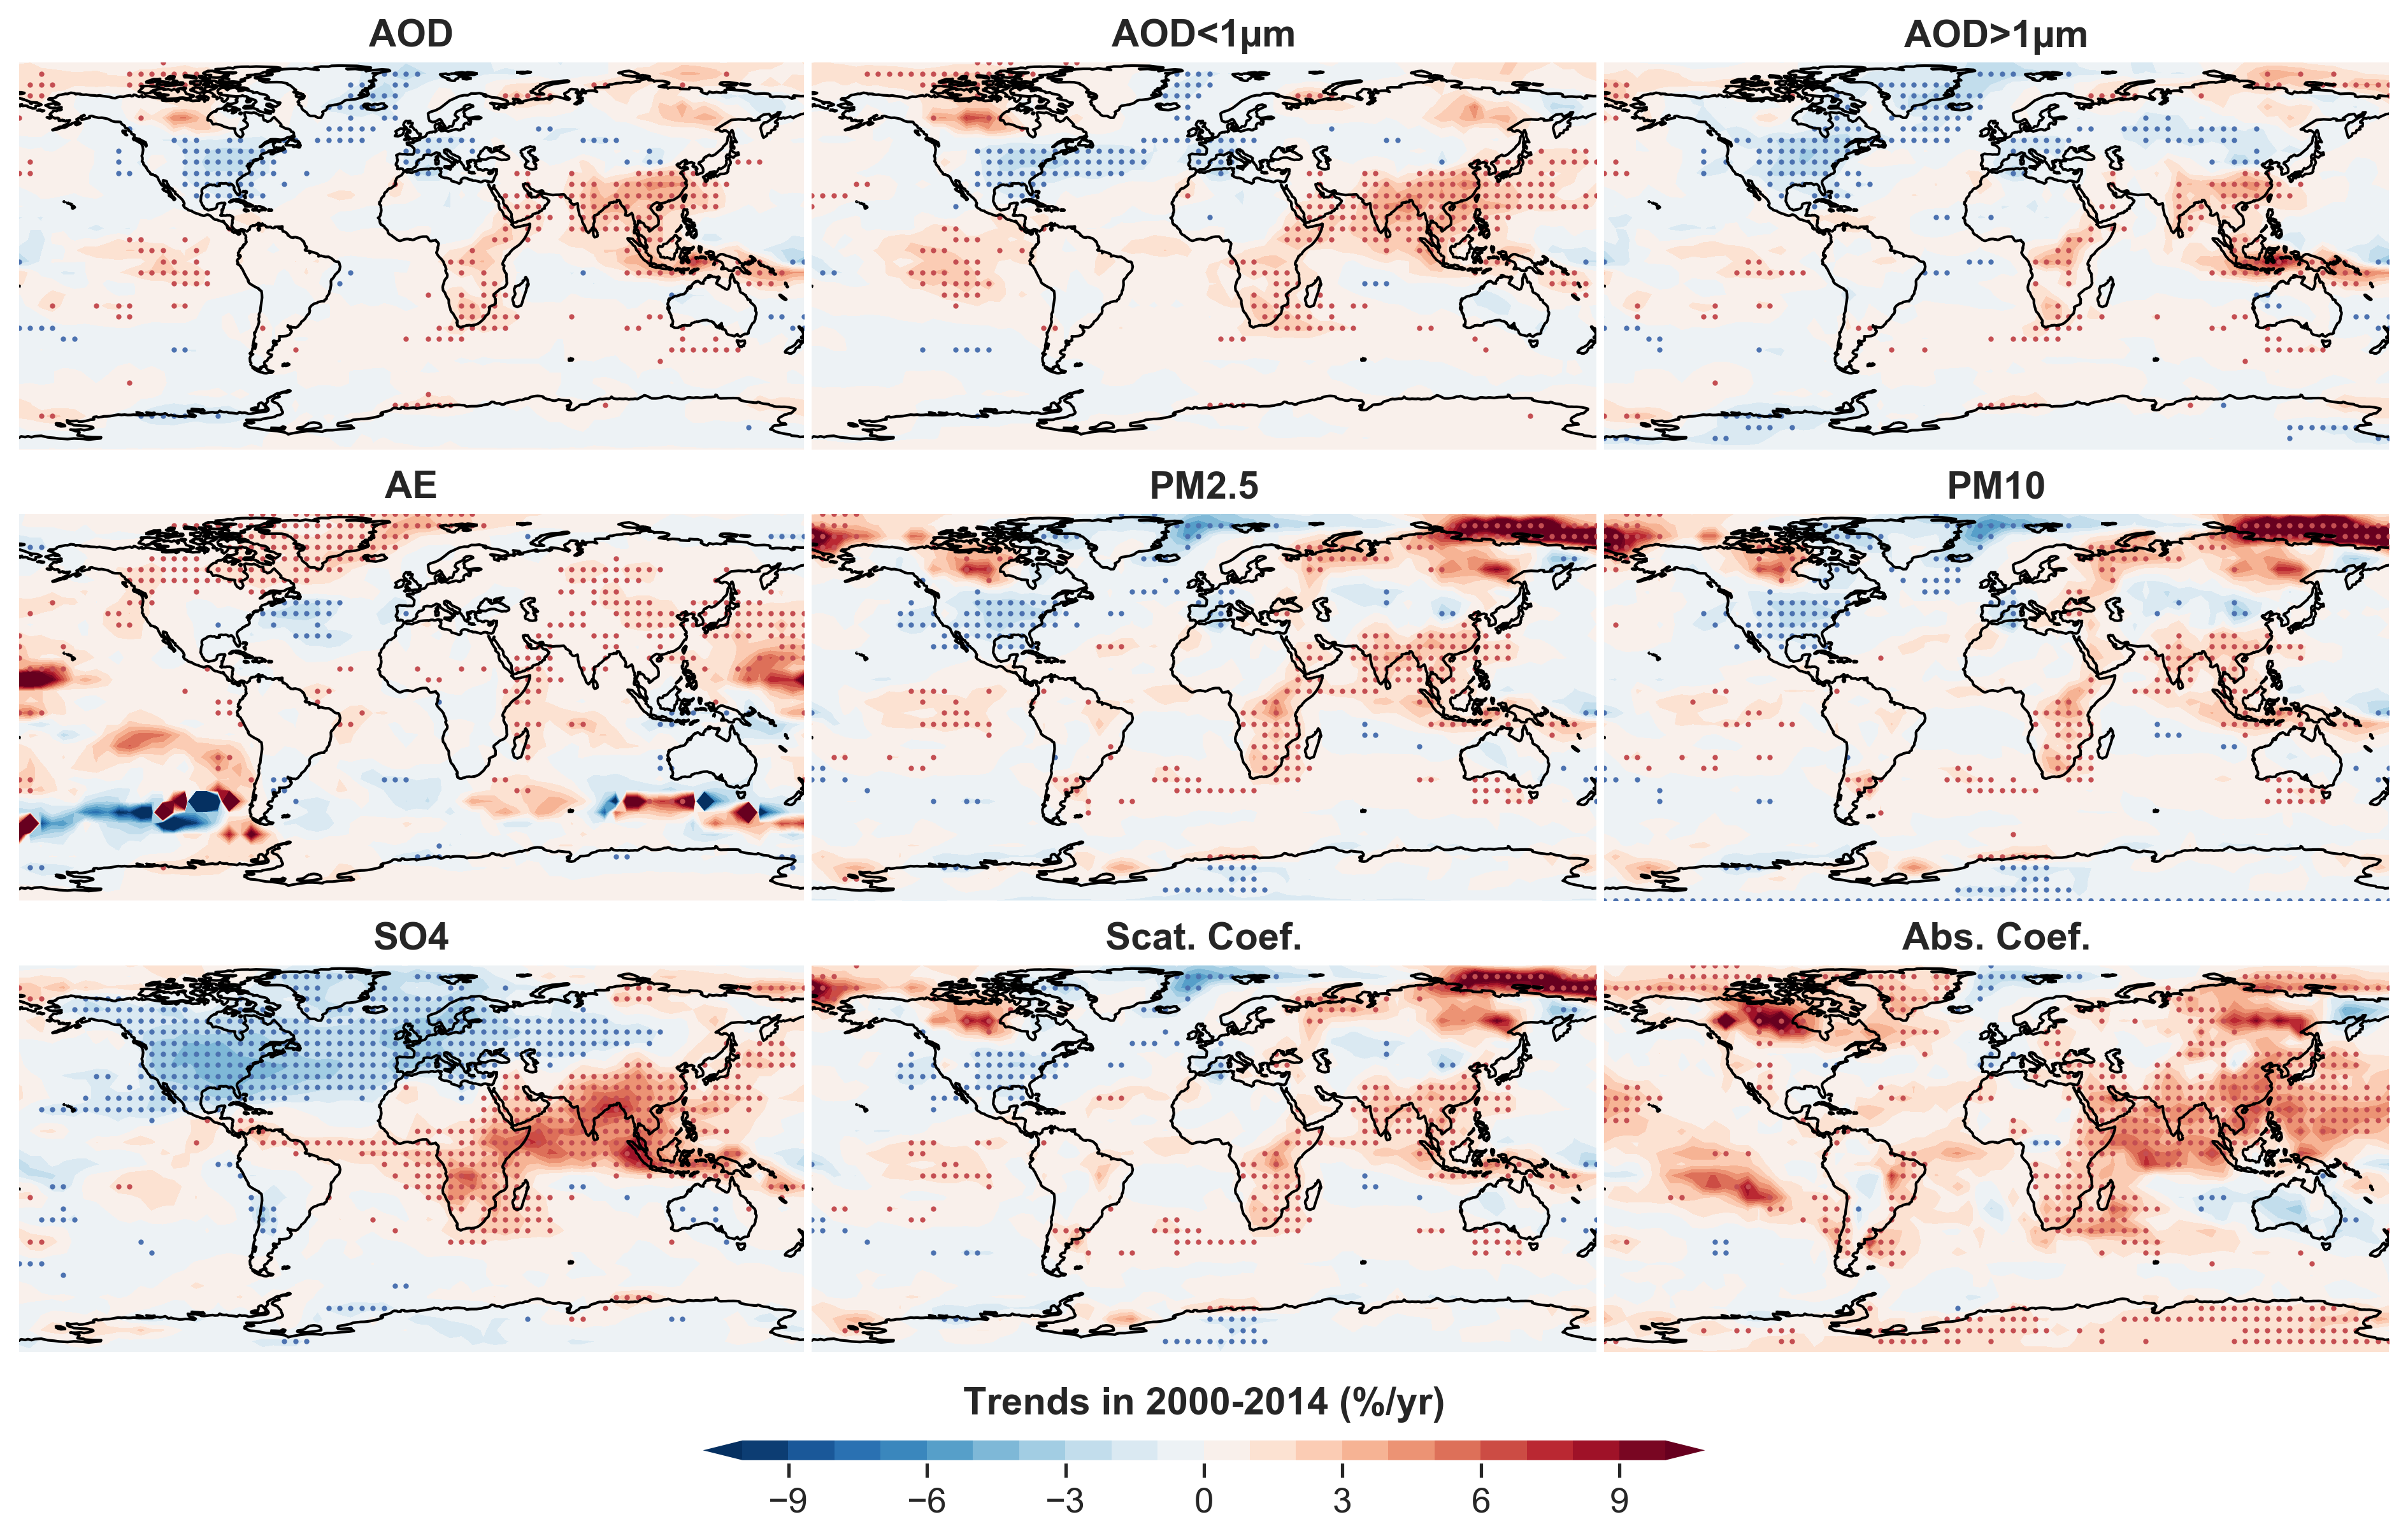
\includegraphics[width=16cm]{../scripts/figs/trends_map2.png}
 \caption{Global trends of aerosol properties using NorESM2 data regridded at a 5x5 degrees resolution. The blue and red dots dots indicate respectively significant negative and positive trends.}
 \label{fig:global_trends}
\end{figure}

As discussed previously, the regional trends presented previously are not always representative of the trends happening in the extended regions and over the whole study period. The reasons are the partial spatial and time coverage of the ground based observations. Moreover, the observation stations are obviously located over land. This does not allow for depiction of a global picture of the aerosol trends, and is unfortunate as sea salt particles are among the most predominant (*reference*) aerosols on Earth.

In order to provide an assessment of the aerosol trends at a global scale, we present, in this section, the trends computed with the NorESM2 data (CMIP6 group) using all grid boxes. The calculation of the global trend is made by averaging the absolute trends computed at each grid-point of the model. In order to provide a relative trend, this absolute trend is normalized to the global average of the considered parameter for the year 2000. The global trends are reported for the nine aerosol parameters in Table \ref{table:global_trends}. The global maps, shown in Figure \ref{fig:global_trends}, enable investigation of the spatial variability of these trends.

While the observed trends of the three AOD parameters show a decrease in most of the regions of the World, the global AOD trend is actually positive (+0.2\%/yr). This global increase is also found with other models. Averages of the models from the CAMS-Rean and the AP3 groups are giving global trends of about +0.2\%/yr and +0.3\%/yr respectively. Within the CMIP6 group, IPSL and CESM2 are also showing positive trends (+0.7\%/yr and +0.3\%/yr), consistently with NorESM2, while CanESM is giving a negative trend (-0.8\%/yr).
This increase of AOD is observed to be larger for the fine fraction, with an increase of about +0.6\%/yr, as compared to +0.1\%/yr for AOD>1µm. As seen in Figure \ref{fig:global_trends}, similar geographical patterns are found for the three AODs: increase in South-Africa and East-Asia and decrease in Europe and in the US. The increasing AOD observed in Canada is dominated by an increase of AOD<1µm in this region. The important increase of AOD in Indonesia seems to be linked to a large increase of AOD>1µm. Over the Pacific Ocean, one region has significant positive modelled trends in both AOD and AOD<1µm. Almost no significant trend is found south of 60\textdegree S.

The model also simulates an increase for AE on a global scale, with a rate of +0.3\%/yr. This suggests a shift towards smaller particles. The largest increases are found over Canada, Greenland, Siberia and the Pacific ocean. There are some distinct outliers around 60\textdegree S. In the Atlantic, we find a decrease of AE, which is consistent with the decrease of AOD<1µm in the same region.

The trends in both $PM_{2.5}$ and $PM_{10}$ exhibit similar geographical features as for AOD. In addition, one finds large and significantly increasing trends in the high Arctic. The global averages show that $PM_{2.5}$ is increasing faster than $PM_{10}$  (+0.2\%/yr vs. +0.1\%/yr), which is consistent with the increasing AE, suggesting a relatively higher fraction of fine particles with time.

The surface $SO_{4}$ concentration trends map reveals two large contrasting regions. Significant decreases are found over North America and Europe, while significant increases are found over southern and eastern Asia and southern to central parts of Africa. This illustrates the shift of polluting activities from the developed countries to the developing countries during the last two decades. With an overall increase of +0.4\%/yr, the global trend is positive.

The Scat. Coef. trends are very similar to those observed for both PM2.5 and PM10. The same geographical patterns are found, as well as the global average trend which amount to an increase of 0.2 \%/yr over the study period.

Abs. Coef. reveals increasing tendencies over most of the grid-boxes of the model, which explains why the largest global trend is obtained for this parameter, with an average of +1.5\%/yr.

Table \ref{table:global_trends} also contains the trends computed for the different aerosol parameters when combining only the grid-points where an observation station is located, whether measurements are available or not. Significant differences can be found when observations are not provided over some regions. This is particularly visible for $SO_{4}$ for which the observation stations are located mostly in Europe and North America, in the large region of decreasing values, while only a few stations are located in the regions associated with increasing values. In this case, the computation of the trends by considering only observation station grid-boxes leads to a global decrease of -1.1\%/yr while the consideration of all of the grid-boxes of the model leads to a global increase of +0.4\%/yr.


\subsubsection{Can we explain the trends in AOD?}

\begin{figure}[t]
 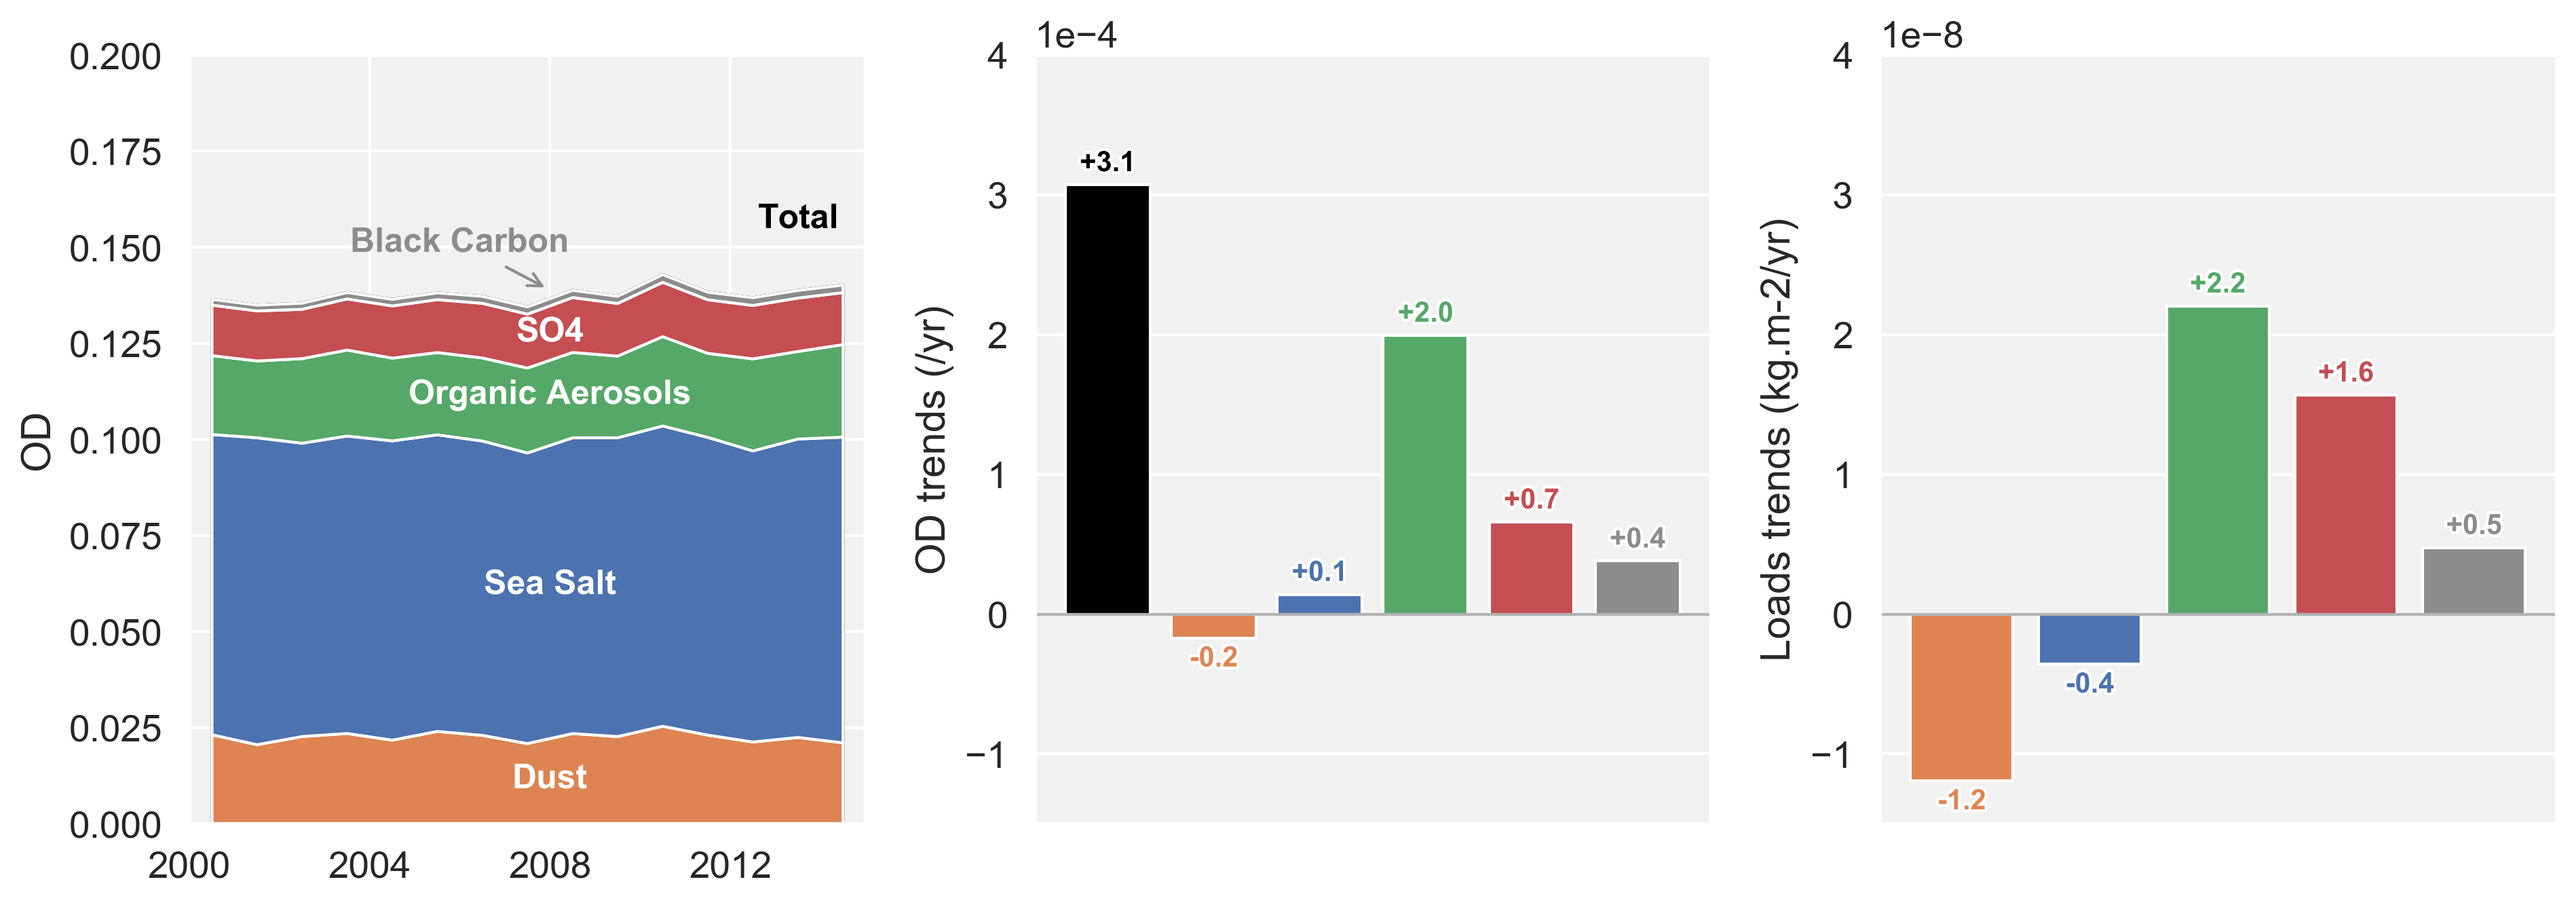
\includegraphics[width=16cm]{../scripts/figs/abs_species_trends.png}
 %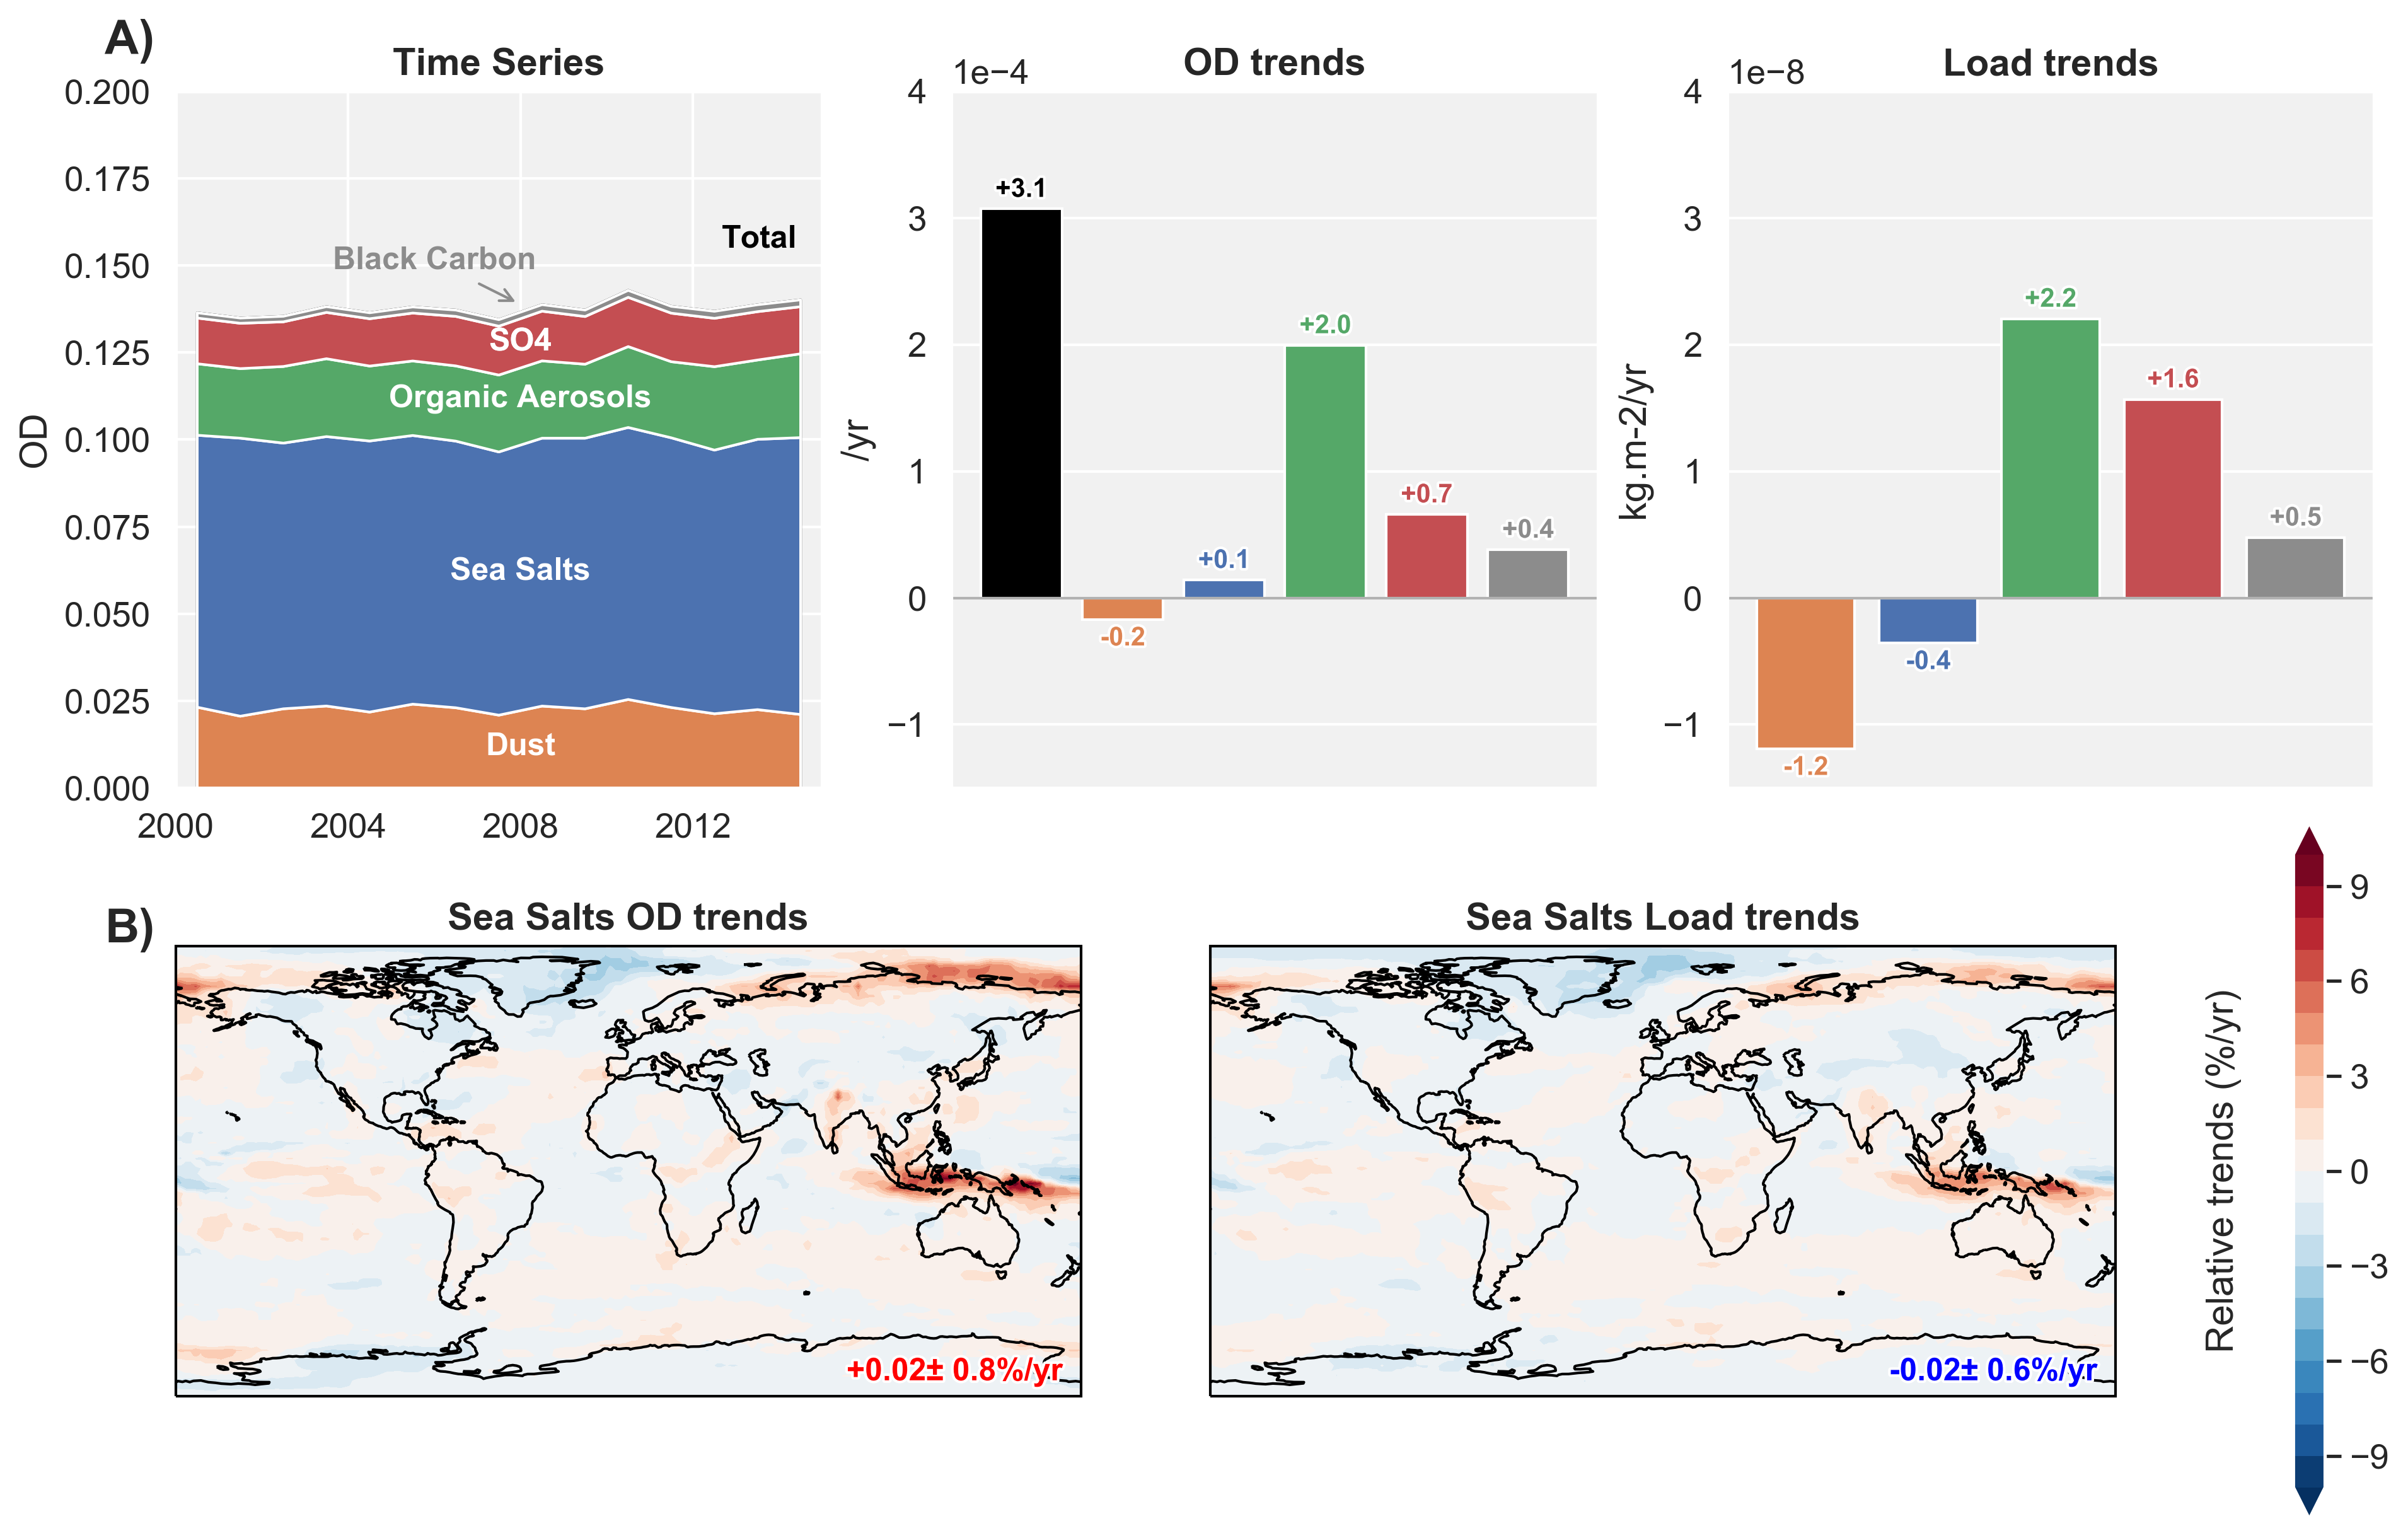
\includegraphics[width=16cm]{../scripts/figs/pannel-abs_species_trends.png}
 \caption{Absolute trends in OD and emissions of the main aerosol species computed with NorESM2. The y-axis of the trends in OD and the emissions is given according to the power of 10 indicated at the top left corner of each of the subplots.}
 \label{fig:species}
\end{figure}

The averaged global trend computed by NorESM2 indicates an increase of AOD in the 2000-2014 period with a rate of about 0.2\%/yr. The trends in AE, AOD<1µm and AOD>1µm indicate that the fine particles are primarily responsible for this increase in the atmospheric column.

In this section, we investigate the trends of the different major aerosol species simulated by NorESM2. For that purpose, the absolute trends of the individual contribution of these species to the AOD were computed, as well as the trends in the loads and the emissions. The trends of OD and loads are shown in Figure \ref{fig:species}.

The relative increase of AOD of +0.2\%/yr corresponds to an absolute increase of +3.1e-4/yr. This positive trend is dominated by an increase of the Organic Aerosols (OA), SO4 and Black Carbon, which are responsible for an increase of the OD of about +2.0e-4/yr, +0.7e-4/yr and +0.4e-4/yr, respectively. On average, the contribution of dust and sea salt is slightly negative (-0.1e-4/yr).

The trends in OD do not necessarily represent the trends in the aerosol loads, since the different species have different Mass Extinction Coefficients (MEC) (dust 1.8 m2.g-1, SS 4.3 m2.g-1, OA 5.6 m2.g-1, SO4 5.3 m2.g-1, BC 7.6 m2.g-1). For sea salt, opposite trends are even observed between OD and the load. The increase of the sea salts load in Indonesia and near the North Pole results in relatively larger increase of OD in these areas. This effect relates to the higher relative humidity at these latitudes which makes the sea salt more efficient at light extinction.


\conclusions  %% \conclusions[modified heading if necessary]

Key points:
\begin{itemize}
 \item The observations highlight mostly negative trends of the extensive parameters in the different regions of the World. In Asia, AE is increasing in time consistently with AOD<1µm and SO4, which probably reflects the regional increase of the anthropogenic aerosols in that region.
 \item Some observation networks allow for derivation of representative trends over the whole period. In other cases, the partial time and space coverage of the observations can induce artificial trends when using regional time series.
 \item The models tend to capture observed AOD, AE and SO4 trends but show larger discrepancies regarding AOD>1μm and PM, compared to measurements.
 \item The global trends computed using model data give a different picture than the trends obtained when using only ground-based observations.
 \item The global trends computed with the model data show mostly positive trends. The trends in AOD are dominated by the increase of the fine particles both in the column and at the surface. This increase appears to be caused by the organic aerosols, for which the emissions have increased in the study period. Also, SO4 OD is increasing as well as its load, even though the emissions did not change significantly.
\end{itemize}

Some perspectives:
\begin{itemize}
 \item  Use of satellites \ref{hsu2012global}:  the averaged AOD trend over global
24 ocean is weakly positive from 1998 to 2010.
 \item What about seasonal trends? For instance, AOD time series for SAMERICA reveal strong cycles for which the local maximum is decreasing significantly in time. The trend could be driven by a decrease of the extreme events *Is it consistent with the expected increasing forest fires?*
 \item also, trends in the meteorological parameters that parameterize the aerosol life cycle and their optical and microphysical properties (wind speed, humidity, temperature)?
 \item What would be the effect of the models trends deviations for the computation of aerosol radiative forcing? \cite{streets2006two,norris2007trends}
\end{itemize}


%% The following commands are for the statements about the availability of data sets and/or software code corresponding to the manuscript.
%% It is strongly recommended to make use of these sections in case data sets and/or software code have been part of your research the article is based on.

\codeavailability{TEXT} %% use this section when having only software code available


\dataavailability{TEXT} %% use this section when having only data sets available


\codedataavailability{TEXT} %% use this section when having data sets and software code available


\sampleavailability{TEXT} %% use this section when having geoscientific samples available


\videosupplement{TEXT} %% use this section when having video supplements available


\appendix
\section{} %\label{sec:representativity} %% Appendix A

\subsection{}     %% Appendix A1, A2, etc.


\noappendix       %% use this to mark the end of the appendix section

%% Regarding figures and tables in appendices, the following two options are possible depending on your general handling of figures and tables in the manuscript environment:

%% Option 1: If you sorted all figures and tables into the sections of the text, please also sort the appendix figures and appendix tables into the respective appendix sections.
%% They will be correctly named automatically.

%% Option 2: If you put all figures after the reference list, please insert appendix tables and figures after the normal tables and figures.
%% To rename them correctly to A1, A2, etc., please add the following commands in front of them:


\appendixfigures  %% needs to be added in front of appendix figures

\appendixtables   %% needs to be added in front of appendix tables

%% Please add \clearpage between each table and/or figure. Further guidelines on figures and tables can be found below.

\begin{table}
 \scriptsize
 \begin{tabularx}{\textwidth}{lX}
  \tophline
  Region    & Sites                                                                                                                                                                                                                                                                                                                                                                                                                                                                                                                                                                                                                                                                                                                                                                                                                                                                                                                                                                                                                                                                                                                                                                                                                                                                                                                                                                                                                                                         \\
  \middlehline
  EUROPE    & Andenes; Arcachon; Aubiere\_LAMP; Autilla; Avignon; BORDEAUX; Barcelona; Bari\_University; Bayfordbury; Belsk; Berlin\_FUB; Birkenes; Brno\_Airport; Brussels; Bucharest\_Inoe; Bure\_OPE; CENER; CLUJ\_UBB; Cabauw; Camborne\_MO; Carpentras; Chilbolton; Coruna; Creteil; Dunkerque; Edinburgh; Eforie; Ersa; FZJ-JOYCE; Fontainebleau; Frioul; Gotland; Hamburg; Helgoland; Helsinki; HohenpeissenbergDWD; Hyytiala; IMAA\_Potenza; ISDGM\_CNR; Iasi\_LOASL; Ispra; Karlsruhe; Kuopio; Kyiv; LAQUILA\_Coppito; Laegeren; Le\_Fauga; Lecce\_University; Leipzig; Lille; Loftus\_MO; Madrid; Magurele\_Inoe; Mainz; Martova; MetObs\_Lindenberg; Minsk; Modena; Moldova; Moscow\_MSU\_MO; Munich\_University; Napoli\_CeSMA; OHP\_OBSERVATOIRE; Oostende; Oxford; Palaiseau; Palencia; Paris; Poprad-Ganovce; Porquerolles; Raciborz; Rame\_Head; Rome\_La\_Sapienza; Rome\_Tor\_Vergata; SMHI; Sevastopol; Seysses; Sirmione\_Museo\_GC; Sodankyla; Strzyzow; The\_Hague; Thessaloniki; Timisoara; Toravere; Toulon; Toulouse\_MF; Valladolid; Venise; Vienna\_UNIVIE; Villefranche; Watnall\_MO; Wytham\_Woods; Xanthi; Zaragoza; Zvenigorod                                                                                                                                                                                                                                                                                                               \\
  ASIA      & Anmyon; Bac\_Giang; Bac\_Lieu; Baengnyeong; Bahrain; Beijing; Beijing-CAMS; Bhola; Chen-Kung\_Univ; Chiang\_Mai\_Met\_Sta; Chiayi; Chiba\_University; Dhabi; Dhadnah; Dhaka\_University; Dongsha\_Island; Dushanbe; EPA-NCU; Fukuoka; Gandhi\_College; Gangneung\_WNU; Gosan\_SNU; Gual\_Pahari; Gwangju\_GIST; Hamim; Hankuk\_UFS; Hokkaido\_University; Hong\_Kong\_PolyU; Hong\_Kong\_Sheung; Irkutsk; Jaipur; Kaashidhoo; Kanpur; Kaohsiung; Karachi; Kuching; Kuwait\_University; Lahore; Luang\_Namtha; Lumbini; MALE; MCO-Hanimaadhoo; Manila\_Observatory; Masdar\_Institute; Mezaira; Mukdahan; Mussafa; NCU\_Taiwan; ND\_Marbel\_Univ; NGHIA\_DO; NhaTrang; Niigata; Nong\_Khai; Noto; Osaka; Pantnagar; Pimai; Pokhara; Pontianak; Pune; Pusan\_NU; Seoul\_SNU; Shirahama; Silpakorn\_Univ; Singapore; Solar\_Village; Son\_La; Songkhla\_Met\_Sta; Tai\_Ping; Taihu; Taipei\_CWB; Tomsk; Tomsk\_22; USM\_Penang; Ubon\_Ratchathani; Ussuriysk; Vientiane; XiangHe; Xinglong; Yekaterinburg; Yonsei\_University                                                                                                                                                                                                                                                                                                                                                                                                                                    \\
  NAMERICA  & ARM\_Oliktok\_AK; Ames; Appledore\_Island; BONDVILLE; Bakersfield; Bermuda; Billerica; Bonanza\_Creek; Bratts\_Lake; Brookhaven; CARTEL; CCNY; COVE; CalTech; Camaguey; Chapais; Chequamegon; Churchill; Columbia\_SC; Dayton; Dry\_Tortugas; EPA-Res\_Triangle\_Pk; Easton-MDE; Easton\_Airport; Egbert; El\_Segundo; Fort\_McKay; Fort\_McMurray; Frenchman\_Flat; Fresno; Fresno\_2; GISS; GSFC; Georgia\_Tech; Grand\_Forks; HJAndrews; Halifax; Harvard\_Forest; Hermosillo; Howland; IMPROVE-MammothCave; Iqaluit; KONZA\_EDC; Kangerlussuaq; Kellogg\_LTER; Kelowna\_UAS; Key\_Biscayne; Key\_Biscayne2; Kuujjuarapik; La\_Jolla; MD\_Science\_Center; Maricopa; Mingo; Missoula; Modesto; Monterey; NASA\_KSC; NASA\_LaRC; NEON-Disney; NEON\_CLBJ; NEON\_GRSM; NEON\_HEAL; NEON\_Harvard; NEON\_KONZ; NEON\_OAES; NEON\_ORNL; NEON\_OSBS; NEON\_SCBI; NEON\_SERC; NEON\_TALL; NEON\_UKFS; NEON\_UNDE; NEON\_WOOD; OPAL; Oyster; PNNL; Pickle\_Lake; Resolute\_Bay; Rimrock; Rogers\_Dry\_Lake; SDSU\_IPLab; SEARCH-Centreville; SEARCH-OLF; SEARCH-Yorkville; SERC; SP\_Bayboro; Sable\_Island; San\_Nicolas; Santa\_Monica\_Colg; Saturn\_Island; Sigma\_Space\_Corp; Sioux\_Falls; St\_Louis\_University; Stennis; Tallahassee; Thompson; Thompson\_Farm; Thule; Toronto; Trinidad\_Head; Tucson; Tudor\_Hill; UAHuntsville; UCLA; UCSB; UH\_Coastal\_Center; UMBC; U\_of\_Wisconsin\_SSEC; Univ\_of\_Houston; Univ\_of\_Lethbridge; Walker\tex... \\
  SAMERICA  & Abracos\_Hill; Alta\_Floresta; Amazon\_ATTO\_Tower; Arica; Balbina; Barbados; Belterra; CEILAP-BA; CEILAP-Bariloche; CEILAP-Comodoro; CEILAP-Neuquen; CEILAP-RG; CUIABA-MIRANDA; Campo\_Grande\_SONDA; Cape\_San\_Juan; Cordoba-CETT; Guadeloup; Itajuba; Ji\_Parana\_SE; La\_Parguera; Manaus\_EMBRAPA; NEON\_GUAN; Petrolina\_SONDA; Pilar\_Cordoba; Puerto\_Madryn; Ragged\_Point; Rio\_Branco; SANTA\_CRUZ; SANTA\_CRUZ\_UTEPSA; San\_Cristobal\_USFQ; Santiago\_Beauchef; Sao\_Martinho\_SONDA; Sao\_Paulo; Surinam; Trelew; Tuxtla\_Gutierrez; UPC-GEAB-Valledupar; UPRM\_Lidar\_Lab; UdeConcepcion-CEFOP                                                                                                                                                                                                                                                                                                                                                                                                                                                                                                                                                                                                                                                                                                                                                                                                                                               \\
  NAFRICA   & ATHENS-NOA; AgiaMarina\_Xyliatou; Agoufou; Badajoz; Banizoumbou; Ben\_Salem; Bidi\_Bahn; Blida; Burjassot; CUT-TEPAK; Cabo\_da\_Roca; Caceres; Cairo\_EMA\_2; DMN\_Maine\_Soroa; Dahkla; Dakar; Djougou; ETNA; Eilat; El\_Arenosillo; El\_Farafra; Evora; FORTH\_CRETE; Gozo; Granada; Hada\_El-Sham; Huelva; IER\_Cinzana; IMC\_Oristano; IMS-METU-ERDEMLI; Ilorin; KAUST\_Campus; Koforidua\_ANUC; Kuwait\_University; LAMTO-STATION; La\_Laguna; Lamezia\_Terme; Lampedusa; Malaga; Medenine-IRA; Messina; Murcia; Nes\_Ziona; Ouagadougou; Oujda; Palma\_de\_Mallorca; Ras\_El\_Ain; SAGRES; SEDE\_BOKER; Saada; Santa\_Cruz\_Tenerife; Solar\_Village; TUBITAK\_UZAY\_Ankara; Tabernas\_PSA-DLR; Technion\_Haifa\_IL; Tizi\_Ouzou; Tunis\_Carthage; Weizmann\_Institute; Zinder\_Airport                                                                                                                                                                                                                                                                                                                                                                                                                                                                                                                                                                                                                                                                 \\
  AUSTRALIA & ARM\_Darwin; Birdsville; Brisbane-Uni\_of\_QLD; Canberra; Darwin; Fowlers\_Gap; Jabiru; Lake\_Argyle; Lake\_Lefroy; Rottnest\_Island; Tinga\_Tingana                                                                                                                                                                                                                                                                                                                                                                                                                                                                                                                                                                                                                                                                                                                                                                                                                                                                                                                                                                                                                                                                                                                                                                                                                                                                                                          \\
  \bottomhline
 \end{tabularx}
 \caption{List of observation stations used for the computation of AOD and AE regional time series.}
 \label{table:stations_aerosun}
\end{table}

\clearpage


\begin{table}
 \scriptsize
 \begin{tabularx}{\textwidth}{lX}
  \tophline
  Region    & Sites                                                                                                                                                                                                                                                                                                                                                                                                                                                                                                                                                                                                                                                                                                                                                                                                                                                                                                                                                                                                                                                                                                                                                                                                                                                                                                                                                                                                                                                                                                                                                   \\
  \middlehline
  EUROPE    & Andenes; Arcachon; Aubiere\_LAMP; Autilla; Bari\_University; Bayfordbury; Belsk; Berlin\_FUB; Birkenes; Brno\_Airport; Brussels; Bucharest\_Inoe; Bure\_OPE; CENER; CLUJ\_UBB; Camborne\_MO; Carpentras; Chilbolton; Coruna; Dunkerque; Edinburgh; Eforie; Ersa; FZJ-JOYCE; Fontainebleau; Frioul; Galata\_Platform; Gloria; Gotland; Gustav\_Dalen\_Tower; Hamburg; Helgoland; Helsinki; Helsinki\_Lighthouse; HohenpeissenbergDWD; Hyytiala; IMAA\_Potenza; ISDGM\_CNR; Iasi\_LOASL; Ispra; Karlsruhe; Kuopio; Kyiv; LAQUILA\_Coppito; Laegeren; Lecce\_University; Leipzig; Lille; Loftus\_MO; Madrid; Magurele\_Inoe; Mainz; Martova; MetObs\_Lindenberg; Minsk; Modena; Moldova; Moscow\_MSU\_MO; Munich\_University; Napoli\_CeSMA; OHP\_OBSERVATOIRE; Oostende; Oxford; Palaiseau; Palencia; Palgrunden; Paris; Poprad-Ganovce; Raciborz; Rame\_Head; Rome\_La\_Sapienza; Rome\_Tor\_Vergata; SMHI; Sevastopol; Sirmione\_Museo\_GC; Sodankyla; Strzyzow; Thessaloniki; Thornton\_C-power; Timisoara; Toravere; Toulon; Toulouse\_MF; Valladolid; Venise; Vienna\_UNIVIE; Watnall\_MO; Wytham\_Woods; Xanthi; Zaragoza; Zeebrugge-MOW1; Zvenigorod                                                                                                                                                                                                                                                                                                                                                                                               \\
  ASIA      & Abu\_Al\_Bukhoosh; Anmyon; Bac\_Giang; Bac\_Lieu; Baengnyeong; Bahrain; Beijing; Beijing-CAMS; Bhola; Chen-Kung\_Univ; Chiang\_Mai\_Met\_Sta; Chiayi; Chiba\_University; Dhabi; Dhadnah; Dhaka\_University; Dongsha\_Island; Dushanbe; EPA-NCU; Fukuoka; GOT\_Seaprism; Gandhi\_College; Gangneung\_WNU; Gosan\_SNU; Gual\_Pahari; Gwangju\_GIST; Hamim; Hankuk\_UFS; Hokkaido\_University; Hong\_Kong\_PolyU; Hong\_Kong\_Sheung; Ieodo\_Station; Irkutsk; Jaipur; Kaashidhoo; Kanpur; Kaohsiung; Karachi; Kuching; Kuwait\_University; Lahore; Luang\_Namtha; Lumbini; MALE; MCO-Hanimaadhoo; Manila\_Observatory; Masdar\_Institute; Mezaira; Mukdahan; Mussafa; NCU\_Taiwan; ND\_Marbel\_Univ; NGHIA\_DO; NhaTrang; Niigata; Nong\_Khai; Noto; Osaka; Pantnagar; Pimai; Pokhara; Pontianak; Pusan\_NU; Seoul\_SNU; Shirahama; Silpakorn\_Univ; Singapore; Socheongcho; Solar\_Village; Son\_La; Songkhla\_Met\_Sta; Tai\_Ping; Taihu; Taipei\_CWB; Tomsk; Tomsk\_22; USM\_Penang; Ubon\_Ratchathani; Ussuriysk; Vientiane; XiangHe; Yekaterinburg; Yonsei\_University                                                                                                                                                                                                                                                                                                                                                                                                                                                                               \\
  NAMERICA  & ARM\_Oliktok\_AK; Ames; Appledore\_Island; BONDVILLE; Bakersfield; Bermuda; Billerica; Bonanza\_Creek; Bratts\_Lake; Brookhaven; CARTEL; CCNY; COVE; COVE\_SEAPRISM; CalTech; Camaguey; Chapais; Chequamegon; Churchill; Columbia\_SC; Dayton; Dry\_Tortugas; EPA-Res\_Triangle\_Pk; Easton-MDE; Easton\_Airport; Egbert; El\_Segundo; Fort\_McKay; Fort\_McMurray; Frenchman\_Flat; Fresno; Fresno\_2; GSFC; Georgia\_Tech; Grand\_Forks; HJAndrews; Halifax; Harvard\_Forest; Hermosillo; Howland; IMPROVE-MammothCave; Iqaluit; KONZA\_EDC; Kangerlussuaq; Kellogg\_LTER; Kelowna\_UAS; Key\_Biscayne; Key\_Biscayne2; Kuujjuarapik; LISCO; La\_Jolla; MD\_Science\_Center; MVCO; Maricopa; Mingo; Missoula; Modesto; Monterey; NASA\_KSC; NASA\_LaRC; NEON-Disney; NEON\_CLBJ; NEON\_GRSM; NEON\_HEAL; NEON\_Harvard; NEON\_KONZ; NEON\_OAES; NEON\_ORNL; NEON\_OSBS; NEON\_SCBI; NEON\_SERC; NEON\_TALL; NEON\_UKFS; NEON\_UNDE; NEON\_WOOD; OPAL; PNNL; Pickle\_Lake; Resolute\_Bay; Rimrock; Rogers\_Dry\_Lake; SDSU\_IPLab; SEARCH-Centreville; SEARCH-OLF; SEARCH-Yorkville; SERC; SP\_Bayboro; Sable\_Island; San\_Nicolas; Santa\_Monica\_Colg; Saturn\_Island; Sigma\_Space\_Corp; Sioux\_Falls; St\_Louis\_University; Stennis; Tallahassee; Thompson; Thompson\_Farm; Thule; Toronto; Trinidad\_Head; Tucson; Tudor\_Hill; UAHuntsville; UCLA; UCSB; UH\_Coastal\_Center; UMBC; USC\_SEAPRISM; USC\_SEAPRISM\_2; U\_of\_Wisconsin\_SSEC; Univ\_of\_Houston; Univ\_of\_Lethbridge; Walker\_Branch; Wallops; Waskesiu; WaveCIS\textunder... \\
  SAMERICA  & Abracos\_Hill; Alta\_Floresta; Amazon\_ATTO\_Tower; Arica; Balbina; Belterra; CEILAP-BA; CEILAP-Bariloche; CEILAP-Comodoro; CEILAP-Neuquen; CEILAP-RG; CUIABA-MIRANDA; Campo\_Grande\_SONDA; Cape\_San\_Juan; Cordoba-CETT; Guadeloup; Itajuba; Ji\_Parana\_SE; La\_Parguera; Manaus\_EMBRAPA; NEON\_GUAN; Petrolina\_SONDA; Pilar\_Cordoba; Puerto\_Madryn; Ragged\_Point; Rio\_Branco; SANTA\_CRUZ; SANTA\_CRUZ\_UTEPSA; San\_Cristobal\_USFQ; Santiago\_Beauchef; Sao\_Martinho\_SONDA; Sao\_Paulo; Trelew; Tuxtla\_Gutierrez; UPC-GEAB-Valledupar; UPRM\_Lidar\_Lab; UdeConcepcion-CEFOP                                                                                                                                                                                                                                                                                                                                                                                                                                                                                                                                                                                                                                                                                                                                                                                                                                                                                                                                                            \\
  NAFRICA   & ATHENS-NOA; AgiaMarina\_Xyliatou; Badajoz; Ben\_Salem; Blida; Burjassot; CUT-TEPAK; Cabo\_da\_Roca; Caceres; Cairo\_EMA\_2; Dahkla; Dakar; ETNA; Eilat; El\_Arenosillo; El\_Farafra; Evora; FORTH\_CRETE; Gozo; Granada; Hada\_El-Sham; IMS-METU-ERDEMLI; Ilorin; KAUST\_Campus; Koforidua\_ANUC; Kuwait\_University; La\_Laguna; Lamezia\_Terme; Lampedusa; Malaga; Murcia; Nes\_Ziona; Oujda; Palma\_de\_Mallorca; SAGRES; SEDE\_BOKER; Santa\_Cruz\_Tenerife; Solar\_Village; TUBITAK\_UZAY\_Ankara; Tabernas\_PSA-DLR; Technion\_Haifa\_IL; Tizi\_Ouzou; Tunis\_Carthage; Weizmann\_Institute                                                                                                                                                                                                                                                                                                                                                                                                                                                                                                                                                                                                                                                                                                                                                                                                                                                                                                                                                       \\
  AUSTRALIA & ARM\_Darwin; Birdsville; Brisbane-Uni\_of\_QLD; Canberra; Darwin; Fowlers\_Gap; Jabiru; Lake\_Argyle; Lake\_Lefroy; Lucinda; Rottnest\_Island; Tinga\_Tingana                                                                                                                                                                                                                                                                                                                                                                                                                                                                                                                                                                                                                                                                                                                                                                                                                                                                                                                                                                                                                                                                                                                                                                                                                                                                                                                                                                                           \\
  \bottomhline
 \end{tabularx}
 \caption{Same as \ref{table:stations_aerosun} for AOD<1µm and AOD>1µm.}
 \label{table:stations_aerosda}
\end{table}

\clearpage

\begin{table}
 \scriptsize
 \begin{tabularx}{\textwidth}{lX}
  \tophline
  Region   & Sites                                                                                                                                                                                                                                                                                                                                                                                                                                                                                                                                                                                                                                                                                                                                                                                                                                                                                                                                                                                                                                                                                                                                                                                                                                                                                                                                                                                                                                                                                                                                                                                                                                                                                                                                                                                                                                                                                                                                                                                                           \\
  \middlehline
  EUROPE   & Aspvreten; Auchencorth Moss; Bilthoven; Birkenes II; Bredkälen; Cabauw Wielsekade; Cabauw Zijdeweg; Cabo de Creus; Chilbolton Observatory; De Zilk; Deuselbach; Diabla Gora; Els Torms; Farkasfa; Guipry; Harwell; Hurdal; Hyytiälä; Illmitz; Iskrba; Ispra; K-puszta; Kollumerwaard; Kosetice (NOAK); Kårvatn; La Coulonche; La Tardière; Lahemaa; Lecce (ECO); Lille Valby; Lista; Mace Head; Melpitz; Montelibretti; Montseny; Morvan; Neuglobsow; Niembro; Norunda Stenen; O Saviñao; Pallas (Matorova); Payerne; Penausende; Peyrusse Vieille; Revin; Rucava; Råö; Saint-Nazaire-le-Désert; Schmücke; Utö; Vavihill; Verneuil; Vilsandi; Vindeln; Virolahti II; Virolahti III; Vredepeel; Waldhof; Zielonka; Zoebelboden; Zoseni                                                                                                                                                                                                                                                                                                                                                                                                                                                                                                                                                                                                                                                                                                                                                                                                                                                                                                                                                                                                                                                                                                                                                                                                                                                                           \\
  NAMERICA & Acadia National Park-McFarland Hill (ME98); Addison Pinnacle; Agua Tibia; Arendtsville (PA00); Atlanta; Badlands NP; Baltimore; Birmingham; Blue Mounds; Bondville (IL11); Boundary Waters Canoe Area; Breton; Bridgton (ME02); Brigantine NWR; Cadiz; Caney Creek; Cape Cod; Cape Romain National Wildlife Refuge; Casco Bay-Wolfe's Neck Farm (ME96); Cedar Bluff; Chassahowitzka National Wildlife Refuge (FL05); Cherokee Nation; Chicago; Cohutta; Columbia Gorge #1; Columbia River Gorge; Connecticut Hill; Death Valley NP; Denali National Park-Mt. McKinley (AK03); Detroit; Dome Lands Wilderness; Egbert; El Dorado Springs; Ellis; Everglades National Park-Research Center (FL11); Fort Peck (IMPROVE); Fresno; Frostberg Reservoir (Big Piney Run); Glacier National Park-Fire Weather Station (MT05); Great Gulf Wilderness; Great River Bluffs; Great Smoky Mountains NP; Hells Canyon; Hercules-Glades; Houston; Isle Royale NP; James River Face Wilderness; Kalmiopsis; Lake Sugema 1; Lake Sugema 2; Linville Gorge; Livonia; Lostwood; M.K. Goddard; Mammoth Cave National Park-Houchin Meadow; Martha's Vineyard; Meadview; Medicine Lake; Mingo; Mohawk Mt.; Moosehorn NWR; Mount Rainier National Park-Tahoma Woods (WA99); Nebraska NF; New York City; North Cascades; Okefenokee National Wildlife Refuge (GA09); Old Town; Olympic; Omaha; Organ Pipe Cactus National Monument; Petersburg; Phoenix; Phoenix Colocated Sampler; Pinnacles National Monument-Bear Valley (CA66); Pittsburgh; Point Reyes National Seashore; Presque Isle; Proctor Maple R. F.; Puget Sound; Quabbin Summit; Quaker City; Queen Valley; Redwood NP; Rubidoux; Sac and Fox; Saguaro NM; Saguaro West; San Rafael; Seney; Sequoia NP; Sikes; Sipsy Wilderness; Spokane Res.; St. Marks; Swanquarter; Tallgrass; Theodore Roosevelt National Park-Painted Canyon; Three Sisters Wilderness; Tonto NM; UL Bend; Upper Buffalo Wilderness; Viking Lake; Voyageurs NP #2; Washington D.C.; Wichita Mount... \\
  \bottomhline
 \end{tabularx}
 \caption{Same as \ref{table:stations_aerosun} for PM2.5}
 \label{table:stations_pm25}
\end{table}

\clearpage

\begin{table}
 \scriptsize
 \begin{tabularx}{\textwidth}{lX}
  \tophline
  Region   & Sites                                                                                                                                                                                                                                                                                                                                                                                                                                                                                                                                                                                                                                                                                                                                                                                                                                                                                                                                                                                                                                                                                                                                                                                                                                                                                                                                                                                                                                                                                                                                                                                                                                                                                                                                                                                                                                                                                                                                                                                                           \\
  \middlehline
  EUROPE   & Aspvreten; Auchencorth Moss; Beromünster; Birkenes II; Braganca; Bredkälen; CEH Edingburgh; Cabauw Wielsekade; Cabo de Creus; Chilbolton Observatory; De Zilk; Deuselbach; Diabla Gora; Eibergen; Els Torms; Farkasfa; Guipry; Harwell; Hohenpeissenberg; Hurdal; Hyytiälä; ISAC Bologna; Illmitz; Iskrba; Ispra; K-puszta; Kamenicki vis; Karpdalen; Keldsnor; Kollumerwaard; Kosetice (NOAK); Kårvatn; La Coulonche; La Tardière; Lahemaa; Lecce (ECO); Leova II; Liesek; Lille Valby; Lough Navar; Mace Head; Melpitz; Montandon; Montelibretti; Montseny; Morvan; Narberth; Neuglobsow; Niembro; Noia; Norunda Stenen; O Saviñao; Pallas (Sammaltunturi); Payerne; Penausende; Peyrusse Vieille; Poiana Stampei; Revin; Risoe; Rucava; Råö; Saint-Nazaire-le-Désert; Schmücke; St. Koloman; Starina; Stará Lesná; Svanvik; Svratouch; Topolniky; Tänikon; University of Gent; Vavihill; Vindeln; Virolahti II; Virolahti III; Vredepeel; Waldhof; Westerland; Zielonka; Zingst; Zoebelboden; Zoseni                                                                                                                                                                                                                                                                                                                                                                                                                                                                                                                                                                                                                                                                                                                                                                                                                                                                                                                                                                                                         \\
  NAMERICA & Acadia National Park-McFarland Hill (ME98); Addison Pinnacle; Agua Tibia; Arendtsville (PA00); Atlanta; Badlands NP; Baltimore; Birmingham; Blue Mounds; Bondville (IL11); Boundary Waters Canoe Area; Breton; Bridgton (ME02); Brigantine NWR; Cadiz; Caney Creek; Cape Cod; Cape Romain National Wildlife Refuge; Casco Bay-Wolfe's Neck Farm (ME96); Cedar Bluff; Chassahowitzka National Wildlife Refuge (FL05); Cherokee Nation; Chicago; Cohutta; Columbia Gorge #1; Columbia River Gorge; Connecticut Hill; Death Valley NP; Denali National Park-Mt. McKinley (AK03); Detroit; Dome Lands Wilderness; Egbert; El Dorado Springs; Ellis; Everglades National Park-Research Center (FL11); Fort Peck (IMPROVE); Fresno; Frostberg Reservoir (Big Piney Run); Glacier National Park-Fire Weather Station (MT05); Great Gulf Wilderness; Great River Bluffs; Great Smoky Mountains NP; Hells Canyon; Hercules-Glades; Houston; Isle Royale NP; James River Face Wilderness; Kalmiopsis; Lake Sugema 1; Lake Sugema 2; Linville Gorge; Livonia; Lostwood; M.K. Goddard; Mammoth Cave National Park-Houchin Meadow; Martha's Vineyard; Meadview; Medicine Lake; Mingo; Mohawk Mt.; Moosehorn NWR; Mount Rainier National Park-Tahoma Woods (WA99); Nebraska NF; New York City; North Cascades; Okefenokee National Wildlife Refuge (GA09); Old Town; Olympic; Omaha; Organ Pipe Cactus National Monument; Petersburg; Phoenix; Phoenix Colocated Sampler; Pinnacles National Monument-Bear Valley (CA66); Pittsburgh; Point Reyes National Seashore; Presque Isle; Proctor Maple R. F.; Puget Sound; Quabbin Summit; Quaker City; Queen Valley; Redwood NP; Rubidoux; Sac and Fox; Saguaro NM; Saguaro West; San Rafael; Seney; Sequoia NP; Sikes; Sipsy Wilderness; Spokane Res.; St. Marks; Swanquarter; Tallgrass; Theodore Roosevelt National Park-Painted Canyon; Three Sisters Wilderness; Tonto NM; UL Bend; Upper Buffalo Wilderness; Viking Lake; Voyageurs NP #2; Washington D.C.; Wichita Mount... \\
  NAFRICA  & Agia Marina Xyliatou ; Cyprus Atmospheric Observatory; Aliartos; Barcarrota; Cairo; Can Llompart; Doñana; Finokalia; Hurghada; Lamezia Terme; Mahón; San Pablo de los Montes; Zarra                                                                                                                                                                                                                                                                                                                                                                                                                                                                                                                                                                                                                                                                                                                                                                                                                                                                                                                                                                                                                                                                                                                                                                                                                                                                                                                                                                                                                                                                                                                                                                                                                                                                                                                                                                                                                             \\
  \bottomhline
 \end{tabularx}
 \caption{Same as \ref{table:stations_aerosun} for PM10}
 \label{table:stations_pm10}
\end{table}

\clearpage

\begin{table}
 \scriptsize
 \begin{tabularx}{\textwidth}{lX}
  \tophline
  Region   & Sites                                                                                                                                                                                                                                                                                                                                                                                                                                                                                                                                                                                                                                                                                                                                                                                                                                                                                                                                                                                                                                                                                                                                                                                                                                                                                                                                                                                                                                                                                                                                                                                                                                                                                                                                                                                                                                                                                                                                                                                                                                                                                                                                                                                                                                                                                                                                                                                                                                                                                                                                                                                                                                                                                                                                                                                                                                                                                                                                                                                                                                                                                                                                                                                                                                                                                                                                                                                                                                                                                                                                                                                                                                                                                                                                                                                                                                                                                                                                                                                                                                                                                                                                                                                                                                                                                    \\
  \middlehline
  EUROPE   & Anholt; Barcombe Mills; Birkenes I and II; Bredkälen; Cabo de Creus; Chopok; Danki; Diabla Gora; Donon; Els Torms; Eskdalemuir; Glen Dye; High Muffles; Hoburgen; Iraty; Iskrba; Ispra; Janiskoski; Jarczew; K-puszta; Kollumerwaard; Kosetice; Kårvatn; La Crouzille; Leba; Logroño; Lough Navar; Melpitz; Montelibretti; Morvan; Niembro; O Saviñao; Osen; Oulanka; Pallas (Matorova); Payerne; Penausende; Peyrusse Vieille; Preila; Rucava; Rörvik-Råö; Sniezka; Strath Vaich Dam; Svratouch; Tange; Tustervatn; Utö; Vavihill; Virolahti; Virolahti II; Vredepeel; Yarner Wood; Ähtäri I-II                                                                                                                                                                                                                                                                                                                                                                                                                                                                                                                                                                                                                                                                                                                                                                                                                                                                                                                                                                                                                                                                                                                                                                                                                                                                                                                                                                                                                                                                                                                                                                                                                                                                                                                                                                                                                                                                                                                                                                                                                                                                                                                                                                                                                                                                                                                                                                                                                                                                                                                                                                                                                                                                                                                                                                                                                                                                                                                                                                                                                                                                                                                                                                                                                                                                                                                                                                                                                                                                                                                                                                                                                                                                                         \\
  ASIA     & Baengnyeong\_Island; Cheju; Chiang Mai (Mae Hia); Hoa Binh; Imsil; Kanghwa; Khanchanaburi (Vachiralongkorn Dam); Listvyanka; Mondy; Oki; Primorskaya; Rishiri; Tanah Rata; Terelj                                                                                                                                                                                                                                                                                                                                                                                                                                                                                                                                                                                                                                                                                                                                                                                                                                                                                                                                                                                                                                                                                                                                                                                                                                                                                                                                                                                                                                                                                                                                                                                                                                                                                                                                                                                                                                                                                                                                                                                                                                                                                                                                                                                                                                                                                                                                                                                                                                                                                                                                                                                                                                                                                                                                                                                                                                                                                                                                                                                                                                                                                                                                                                                                                                                                                                                                                                                                                                                                                                                                                                                                                                                                                                                                                                                                                                                                                                                                                                                                                                                                                                        \\
  NAMERICA & Abington; Acadia NP; Acadia\_NP; Addison\_Pinnacle; Agua\_Tibia; Algoma; Alhambra; Ann Arbor; Arches\_NP; Arendtsville; Ashland; Badlands\_NP; Bandelier\_NM; Barrier\_Lake; Beaufort; Beltsville; Big Bend NP; Big\_Bend\_NP; Blackwater NWR; Bliss\_SP\_(TRPA); Blue\_Mounds; Bondville; Bosque\_del\_Apache; Boulder\_Lake; Boundary\_Waters\_Canoe\_Area; Breton; Breton\_Island; Bridger\_Wilderness; Bridgton; Brigantine\_NWR; Brooklyn\_Lake; Bryce\_Canyon\_NP; Cabinet\_Mountains; Caddo Valley; Cadiz; Candor; Caney\_Creek; Canyonlands NP; Canyonlands\_NP; Cape\_Cod; Cape\_Romain\_NWR; Capitol\_Reef\_NP; Casco\_Bay; Cedar Creek; Cedar\_Bluff; Centennial; Chalk River; Chapais; Chassahowitzka\_NWR; Cherokee\_sNation; Chiricahua NM; Chiricahua\_NM; Claryville; Cloud\_Peak; Coffeeville; Cohutta; Columbia\_Gorge\_#1; Columbia\_River\_Gorge; Connecticut Hill; Connecticut\_Hill; Coweeta; Cranberry; Crater\_Lake\_NP; Craters\_of\_the\_Moon\_NM; Crescent\_Lake; Crockett; Death\_Valley\_NP; Deer Creek; Denali NP; Denali\_NP; Dolly\_Sods\_Wilderness; Dome\_Lands\_Wilderness; Douglas; E.L.A.; Edgar Evins; Egbert; El\_Dorado\_Springs; Ellis; Everglades NP; Everglades\_NP; Flat\_Tops; Flathead; Fort\_Peck; Frostberg\_Reservoir\_(Big\_Piney\_Run); Gates\_of\_the\_Mountains; Georgia Station; Gila\_Wilderness; Glacier NP; Glacier\_NP; Gothic; Grand Canyon NP; Great Basin NP; Great Smoky NP - Look Rock; Great\_Basin\_NP; Great\_Gulf\_Wilderness; Great\_River\_Bluffs; Great\_Sand\_Dunes\_NM; Great\_Smoky\_Mountains\_NP; Guadalupe\_Mountains\_NP; Hance\_Camp\_at\_Grand\_Canyon\_NP; Hells\_Canyon; Hercules-Glades; Hillside; Hoover; Hopi\_Point\_#1; Horton Station; Howland; Hoxeyville; Ike's\_Backbone; Indian\_Gardens; Isle\_Royale\_NP; James\_River\_Face\_Wilderness; Jarbidge\_Wilderness; Jefferson\_NF; Joshua Tree NP; Joshua\_Tree\_NP; Kaiser; Kalmiopsis; Kane Exp. Forest; Kejimkujik; Lake\_Sugema; Lake\_Tahoe\_Community\_College; Lassen Volcanic NP; Lassen\_Volcanic\_NP; Laurel Hill; Lava\_Beds\_NM; Linville\_Gorge; Livonia; Londonderry; Lone\_Peak\_Wilderness; Longwoods; Lostwood; Lye\_Brook\_Wilderness; Lykens; Lynden; M.K. Goddard; M.K.\_Goddard; Mackville; Mackville Collocated; Makah\_Tribe; Makah\_Tribe\_Site\_#2; Mammoth\_Cave\_NP; Martha's\_Vineyard; Meadview; Medicine\_Lake; Mesa Verde NP; Mesa\_Verde\_NP; Mingo; Mohawk\_Mt.; Monture; Moosehorn\_NWR; Mount Rainier NP; Mount\_Baldy; Mount\_Hood; Mount\_Rainier\_NP; Mount\_Zirkel\_Wilderness; Nebraska\_NF; North\_Absaroka; North\_Cascades; Northern\_Cheyenne; Okefenokee\_NWR; Old\_Town; Olympic; Omaha; Organ\_Pipe; Owens\_Valley; Oxford; Pack\_Monadnock\_Summit; Parsons; Pasayten; Penn State; Penobscot; Perkinstown; Petersburg; Petrified\_Forest\_NP; Pinedale; Pinnacles NM; Pinnacles\_NM; Point\_Reyes\_National\_Seashore; Presque\_Isle; Prince Edward; Proctor\_Maple\_R.\_F.; Quabbin\_Summit; Quaker City; Quaker\_City; Queen\_Valley; Redwood\_NP; Ripple\_Creek; Rocky Mtn NP; Rocky\_Mountain\_NP; Rocky\_Mountain\_NP\_HQ; Sac\_and\_Fox; Saguaro\_NM; Saguaro\_West; Salamonie Reservoir; Salmon\_NF; Salt\_Creek; San\_Andres; San\_Gabriel; San\_Gorgonio\_Wilderness; San\_Pedro\_Parks; San\_Rafael; Sand Mountain; Saturna; Sawtooth\_NF; Scoville; Seney; Sequoia\_NP; Shamrock\_Mine; Shenandoah NP - Big Meadows; Shenandoah\_NP; Shining\_Rock\_Wilderness; Sierra\_Ancha; Sikes; Sipsey\_Wilderness; Snoqualmie\_Pass; South\_Lake\_Tahoe; Speedwell; Spokane\_Res.; St.\_Marks; Starkey; Stilwell; Stockton; Storm\_Peak; Sula\_Peak; Sumatra; Swanquarter; Sycamore\_Canyon; Tallgrass; Theodore Roosevelt NP; Theodore\_Roosevelt; Three\_Sisters\_Wilderness; Thunder\_Basin; Tonto\_NM; Trinity; UL\_Bend; Unionville; Upper\_Buffalo\_Wilderness; Viking\_Lake; Vincennes; Voyageurs NP; Voyageurs\_NP\_#1; Voyageurs\_NP\_#2; WY; Walker\_River\_Paiute\_Tribe; Wash. Crossing; Weminuche\_Wilderness; Wheeler\_Peak; White\_Mountain; White\_Pass; White\_River\_NF; Whiteface Mountain; Wichita\_Mountains; Wind\_Cave; Woodstock; Wrightwood; Yellowstone NP; Yellowstone\_NP\_1; Yellowstone\_NP\_2; Yosemite NP - Turtleback Dome; Yosemite\_NP; Zion; Zion\_Canyon \\
  NAFRICA  & Barcarrota; Víznar; Zarra                                                                                                                                                                                                                                                                                                                                                                                                                                                                                                                                                                                                                                                                                                                                                                                                                                                                                                                                                                                                                                                                                                                                                                                                                                                                                                                                                                                                                                                                                                                                                                                                                                                                                                                                                                                                                                                                                                                                                                                                                                                                                                                                                                                                                                                                                                                                                                                                                                                                                                                                                                                                                                                                                                                                                                                                                                                                                                                                                                                                                                                                                                                                                                                                                                                                                                                                                                                                                                                                                                                                                                                                                                                                                                                                                                                                                                                                                                                                                                                                                                                                                                                                                                                                                                                                \\
  \bottomhline
 \end{tabularx}
 \caption{Same as \ref{table:stations_aerosun} for SO4 concentration}
 \label{table:stations_so4}
\end{table}

\clearpage

\begin{table}
 \scriptsize
 \begin{tabularx}{\textwidth}{lX}
  \tophline
  Region   & Sites                                                                                                                                                                                                                                                                                                                                                                                                                                                                                                                                                                                \\
  \middlehline
  EUROPE   & Birkenes II; Cabauw Zijdeweg; Hohenpeissenberg; Hyytiälä; K-puszta; Kosetice (NOAK); Mace Head; Melpitz; Observatoire Perenne de l'Environnement; Pallas (Sammaltunturi); Vavihill                                                                                                                                                                                                                                                                                                                                                                                                   \\
  NAMERICA & Acadia National Park-McFarland Hill (ME98); Bondville; Boundary Waters Canoe Area; Cedar Bluff; Columbia River Gorge; Glacier National Park-Fire Weather Station (MT05); Great Gulf Wilderness; Great Smoky Mountains NP; James River Face Wilderness; Mammoth Cave National Park-Houchin Meadow; Mount Rainier National Park-Tahoma Woods (WA99); Okefenokee National Wildlife Refuge (GA09); Organ Pipe Cactus National Monument; Saguaro NM - Tucson Mountain #1; Southern Great Plains E13; Three Sisters Wilderness; Trinidad Head; Upper Buffalo Wilderness; Wichita Mountains \\
  \bottomhline
 \end{tabularx}
 \caption{Same as \ref{table:stations_aerosun} for Scat. Coef.}
 \label{table:stations_scat}
\end{table}

\clearpage

\begin{table}
 \scriptsize
 \begin{tabularx}{\textwidth}{lX}
  \tophline
  Region   & Sites                                                                                                                                                                                                                                                                                                                                                                            \\
  \middlehline
  EUROPE   & Annaberg-Buchholz; Aspvreten; Birkenes II; Bösel; Cabauw Zijdeweg; Harwell; Hohenpeissenberg; Hyytiälä; Ispra; K-puszta; Kosetice (NOAK); Leipzig; Leipzig-Eisenbahnstrasse; Leipzig-West; Mace Head; Melpitz; Montseny; Neuglobsow; Observatoire Perenne de l'Environnement; Pallas (Sammaltunturi); SIRTA Atmospheric Research Observatory; Vavihill; Waldhof; Ústí n.L.-mesto \\
  NAMERICA & Bondville; Sable Island; Southern Great Plains E13; Trinidad Head                                                                                                                                                                                                                                                                                                                \\
  \bottomhline
 \end{tabularx}
 \caption{Same as \ref{table:stations_aerosun} for Abs. Coef.}
 \label{table:stations_abs}
\end{table}


\authorcontribution{TEXT} %% this section is mandatory

\competinginterests{TEXT} %% this section is mandatory even if you declare that no competing interests are present

\disclaimer{TEXT} %% optional section

\begin{acknowledgements}
 TEXT
\end{acknowledgements}




%% REFERENCES

%% The reference list is compiled as follows:

%\begin{thebibliography}{}

% \bibitem[AUTHOR(YEAR)]{LABEL1}
% REFERENCE 1

% \bibitem[AUTHOR(YEAR)]{LABEL2}
% REFERENCE 2

%\end{thebibliography}

%% Since the Copernicus LaTeX package includes the BibTeX style file copernicus.bst,
%% authors experienced with BibTeX only have to include the following two lines:
%%
\bibliographystyle{copernicus}
\bibliography{mybib.bib}
%%
%% URLs and DOIs can be entered in your BibTeX file as:
%%
%% URL = {http://www.xyz.org/~jones/idx_g.htm}
%% DOI = {10.5194/xyz}


%% LITERATURE CITATIONS
%%
%% command                        & example result
%% \citet{jones90}|               & Jones et al. (1990)
%% \citep{jones90}|               & (Jones et al., 1990)
%% \citep{jones90,jones93}|       & (Jones et al., 1990, 1993)
%% \citep[p.~32]{jones90}|        & (Jones et al., 1990, p.~32)
%% \citep[e.g.,][]{jones90}|      & (e.g., Jones et al., 1990)
%% \citep[e.g.,][p.~32]{jones90}| & (e.g., Jones et al., 1990, p.~32)
%% \citeauthor{jones90}|          & Jones et al.
%% \citeyear{jones90}|            & 1990



%% FIGURES

%% When figures and tables are placed at the end of the MS (article in one-column style), please add \clearpage
%% between bibliography and first table and/or figure as well as between each table and/or figure.


%% ONE-COLUMN FIGURES

%%f
%\begin{figure}[t]
%\includegraphics[width=12cm]{FILE NAME}
%\caption{TEXT}
%\end{figure}
%
%%% TWO-COLUMN FIGURES
%
%%f
%\begin{figure*}[t]
%\includegraphics[width=16cm]{FILE NAME}
%\caption{TEXT}
%\end{figure*}
%
%
%%% TABLES
%%%
%%% The different columns must be seperated with a & command and should
%%% end with \\ to identify the column brake.
%
%%% ONE-COLUMN TABLE
%
%%t
%\begin{table}[t]
%\caption{TEXT}
%\begin{tabular}{column = lcr}
%\tophline
%
%\middlehline
%
%\bottomhline
%\end{tabular}
%\belowtable{} % Table Footnotes
%\end{table}
%
%%% TWO-COLUMN TABLE
%
%%t
%\begin{table*}[t]
%\caption{TEXT}
%\begin{tabular}{column = lcr}
%\tophline
%
%\middlehline
%
%\bottomhline
%\end{tabular}
%\belowtable{} % Table Footnotes
%\end{table*}
%
%%% LANDSCAPE TABLE
%
%%t
%\begin{sidewaystable*}[t]
%\caption{TEXT}
%\begin{tabular}{column = lcr}
%\tophline
%
%\middlehline
%
%\bottomhline
%\end{tabular}
%\belowtable{} % Table Footnotes
%\end{sidewaystable*}
%
%
%%% MATHEMATICAL EXPRESSIONS
%
%%% All papers typeset by Copernicus Publications follow the math typesetting regulations
%%% given by the IUPAC Green Book (IUPAC: Quantities, Units and Symbols in Physical Chemistry,
%%% 2nd Edn., Blackwell Science, available at: http://old.iupac.org/publications/books/gbook/green_book_2ed.pdf, 1993).
%%%
%%% Physical quantities/variables are typeset in italic font (t for time, T for Temperature)
%%% Indices which are not defined are typeset in italic font (x, y, z, a, b, c)
%%% Items/objects which are defined are typeset in roman font (Car A, Car B)
%%% Descriptions/specifications which are defined by itself are typeset in roman font (abs, rel, ref, tot, net, ice)
%%% Abbreviations from 2 letters are typeset in roman font (RH, LAI)
%%% Vectors are identified in bold italic font using \vec{x}
%%% Matrices are identified in bold roman font
%%% Multiplication signs are typeset using the LaTeX commands \times (for vector products, grids, and exponential notations) or \cdot
%%% The character * should not be applied as mutliplication sign
%
%
%%% EQUATIONS
%
%%% Single-row equation
%
%\begin{equation}
%
%\end{equation}
%
%%% Multiline equation
%
%\begin{align}
%& 3 + 5 = 8\\
%& 3 + 5 = 8\\
%& 3 + 5 = 8
%\end{align}
%
%
%%% MATRICES
%
%\begin{matrix}
%x & y & z\\
%x & y & z\\
%x & y & z\\
%\end{matrix}
%
%
%%% ALGORITHM
%
%\begin{algorithm}
%\caption{...}
%\label{a1}
%\begin{algorithmic}
%...
%\end{algorithmic}
%\end{algorithm}
%
%
%%% CHEMICAL FORMULAS AND REACTIONS
%
%%% For formulas embedded in the text, please use \chem{}
%
%%% The reaction environment creates labels including the letter R, i.e. (R1), (R2), etc.
%
%\begin{reaction}
%%% \rightarrow should be used for normal (one-way) chemical reactions
%%% \rightleftharpoons should be used for equilibria
%%% \leftrightarrow should be used for resonance structures
%\end{reaction}
%
%
%%% PHYSICAL UNITS
%%%
%%% Please use \unit{} and apply the exponential notation


\end{document}
